\documentclass[11pt,class=report,crop=false]{standalone}
\usepackage[screen]{../mathgame}
%\usepackage{xinttools}

\begin{document}


%====================================================================
\chapitre{Mouvement}
%====================================================================

%
%\insertvideo{yUgpElITYTg}{partie 5.1. Bits classiques}
%
%\insertvideo{iET0snUXj0k}{partie 5.2. Portes logiques}
%
%\insertvideo{JKmC2u5kvKg}{partie 5.3. Algorithme et complexité}


\objectifs{Comment se déplacer dans le plan, dans l'espace, dans un labyrinthe, sur un terrain ?}

%%%%%%%%%%%%%%%%%%%%%%%%%%%%%%%%%%%%%%%%%%%%%%%%%%%%%%%%%%%%%%%%%%%%%
\section{Position, vitesse, accélération}

%--------------------------------------------------------------------
\subsection{Position}

\textbf{Déplacement via les coordonnées cartésiennes.}
Dans le plan on repère la position d'un objet ponctuel par deux coordonnées $P = (x,y)$.
Pour se déplacer, on peut indiquer le vecteur déplacement souhaité $\vec v = (v_x,v_y)$.
Le nouveau point est :
$$P' = P + \vec{v} = (x+v_x, y + v_y).$$

\myfigure{0.7}{
	\tikzinput{fig-position-01}
}
	
Autrement dit, pour aller du point $P_1 = (x_1,y_1)$ au point $P_2 = (x_2,y_2)$, le vecteur correspondant est :
$$\vec v  = P_2 - P_1 = (x_2-x_1, y_2-y_1).$$


\textbf{Déplacement via les coordonnées polaires.} 
On pourrait aussi repérer $\vec v$ par ses coordonnées polaires $[r:\theta]$ c'est-à-dire
$\vec v  = (r\cos \theta, r\sin\theta)$.

\myfigure{0.7}{
	\tikzinput{fig-position-02}
}

\textbf{Déplacement en mode \og{}tortue\fg{}.} 
On repère une tortue en déplacement (comme dans le logiciel \emph{Scratch}) par sa position actuelle $P$ et sa direction $\vec u$.
\begin{itemize}
	\item L'instruction \emph{avancer} correspond à déplacer la tortue au point $P' = P  + \delta \vec u$ où $\delta$ correspond à un nombre de pas par exemple.

    \item L'instruction \emph{tourner} correspond à changer le vecteur de direction $\vec u$, en lui appliquant une rotation d'angle $\theta$.
    Si $\vec u$ est un vecteur unitaire (c'est-à-dire $\| \vec u \| = 1$) alors le nouveau vecteur de direction est :    
    $$\vec{u'} = \vec{u} + (\cos \theta, \sin\theta).$$
\end{itemize}

\myfigure{0.7}{
	\tikzinput{fig-tortue-01}\quad
	\tikzinput{fig-tortue-02}\quad
	\tikzinput{fig-tortue-03}		
}

\textbf{Dans l'espace.}
Nous avons besoin de trois coordonnées $P = (x,y,z)$ et $\vec v = (v_x,v_y,v_z)$ et alors $P' = P + \vec v = (x+v_x, y+v_y, z+v_z)$.
Pour comprendre comment se déplacer en mode \og{}tortue\fg{} dans l'espace, on renvoie au chapitre \og{}Fractales\fg{}.


%--------------------------------------------------------------------
\subsection{Vitesse}

Considérons un point $P(t)$ en mouvement en fonction d'un paramètre de temps $t \in \Rr$. La \defi{vitesse}\index{vitesse} $\vec{v}(t)$ est définie comme la dérivée de la position par rapport au temps :
$$\vec{v}(t) = \frac{\dd P(t)}{\dd t}.$$
Le vecteur vitesse $\vec{v}(t)$ est tangent à la trajectoire en $P(t)$ et plus la particule se déplace vite, plus sa longueur est grande.

\myfigure{1}{
	\tikzinput{fig-position-03}
}


Si la position $P(t)$ est donnée en coordonnées par $(x(t),y(t))$, calculer le vecteur dérivé revient à dériver chacune des fonctions $t \mapsto x(t)$ et $t \mapsto y(t)$ :
$$\vec{v}(t) = (x'(t), y'(t)).$$

Pour estimer cette vitesse instantanée on peut calculer une vitesse moyenne sur un intervalle de temps $\dd t$ très court :
$$\vec{v}(t) \simeq \frac{P(t + \dd t) - P(t)}{\dd t}.$$
Cette formule correspond à la définition de la dérivée comme une limite.

Remarque : un meilleure approximation peut être obtenue par la formule :
$$\vec{v}(t) \simeq \frac{P(t + \dd t) - P(t-\dd t)}{2\dd t}.$$

\myfigure{1}{
	\tikzinput{fig-position-04}
}

%--------------------------------------------------------------------
\subsection{Accélération}

L'\defi{accélération}\index{acceleration@accélération} est la dérivée de la vitesse :
$$\vec{a}(t) = \frac{\dd \vec{v}(t)}{\dd t}.$$

En coordonnées : $\vec{a}(t) = (x''(t), y''(t))$.


Par exemple, un objet soumis à aucune force aura une accélération égale au vecteur nul et se déplace suivant un mouvement rectiligne uniforme : son vecteur vitesse est constant $\vec v(t) = \vec{v_0}$ et sa position à l'instant $t$ sera $P(t) = P(0) + t \vec{v_0}$.


%--------------------------------------------------------------------
\subsection{Courbe de poursuite}

Tracer des courbes de poursuite est un petit exercice de programmation amusant.
Un chat $C$ court après une souris $S$. 
La souris a une trajectoire $S(t)$ et à tout instant le chat se dirige vers la souris. Tracer la trajectoire $C(t)$ du chat.


\begin{center}
	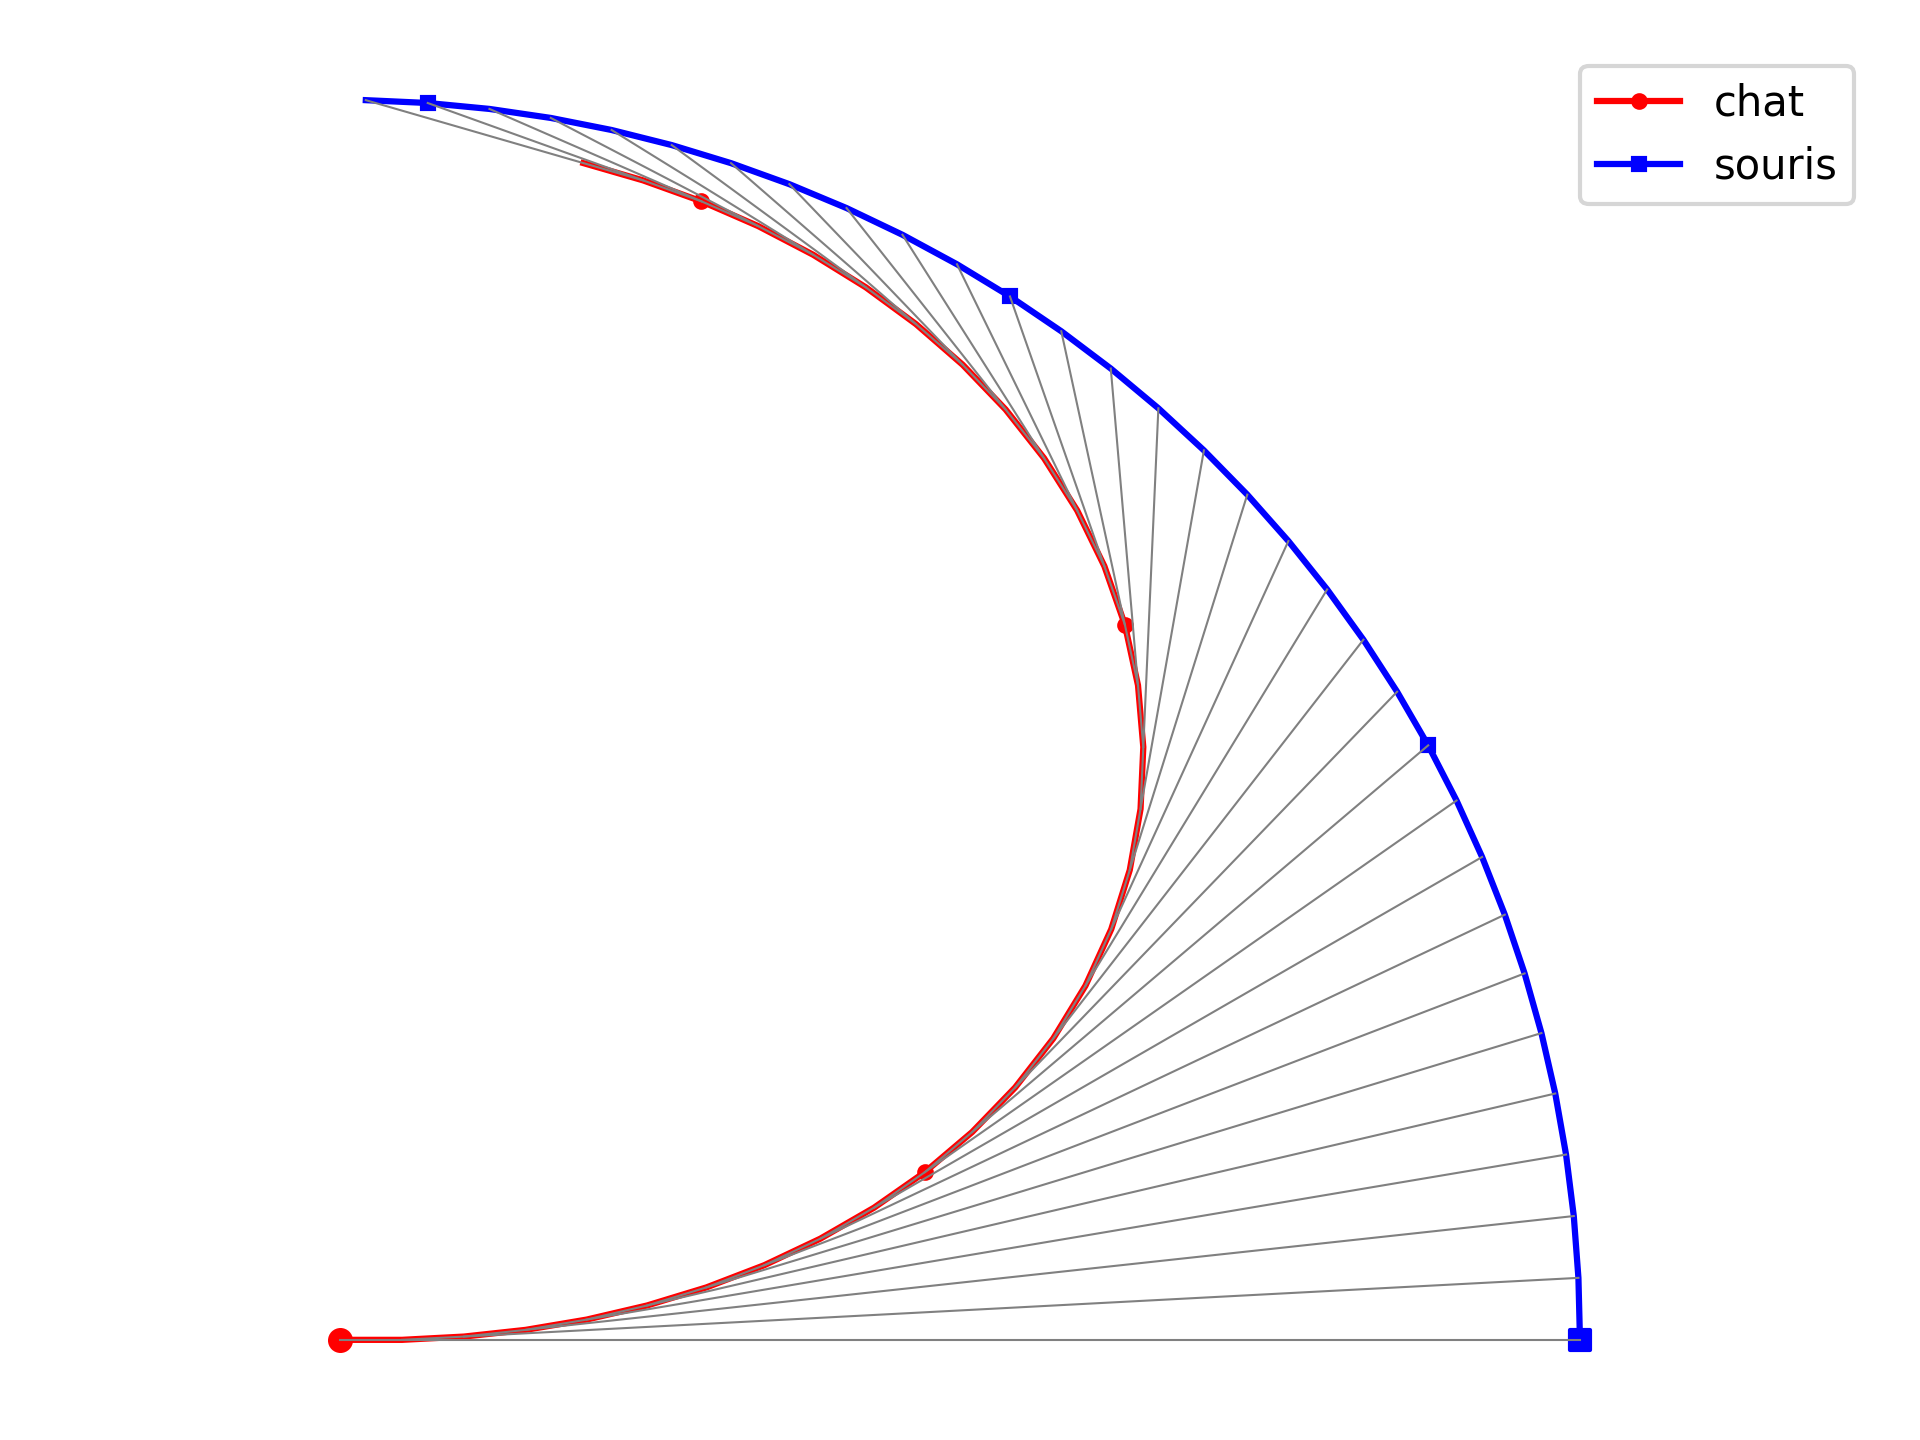
\includegraphics[scale=\myscale,scale=0.45]{figures/poursuite-01}\qquad\qquad
	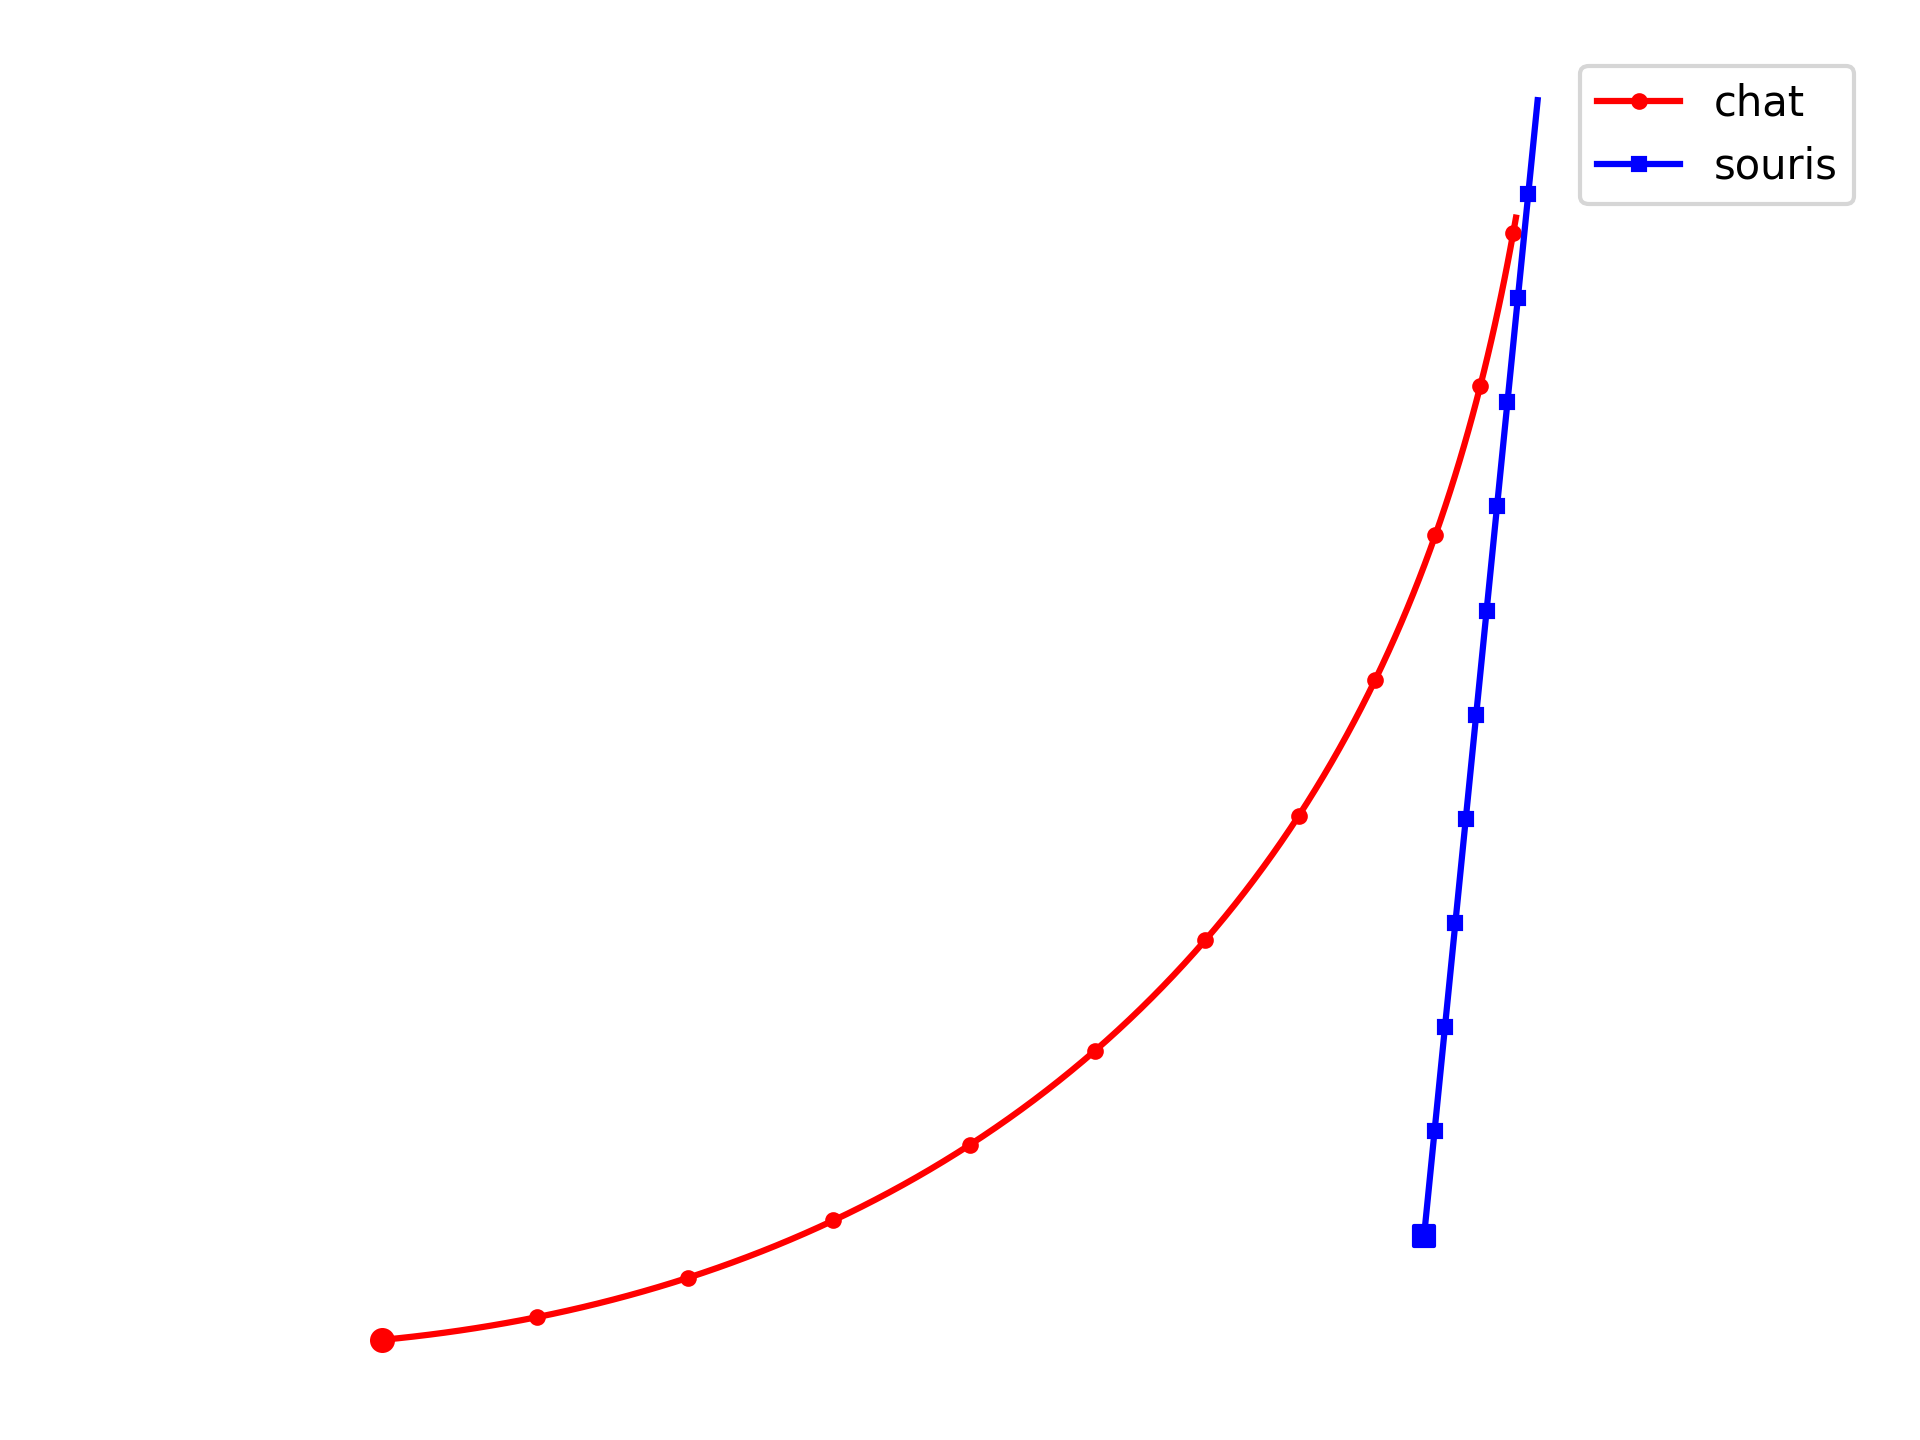
\includegraphics[scale=\myscale,scale=0.45]{figures/poursuite-02}
\end{center}

Les données et les étapes sont les suivantes:
\begin{itemize}
	\item se donner une trajectoire $S(t)$ pour la souris,
	\item se donner une position initiale $C(0)$ du chat, 
	\item se donner un réel $v$ pour la norme de la vitesse du chat,
	\item définir un intervalle élémentaire de temps $\dd t$ (par exemple $\dd t = 0.1$),
	
	\item faire une boucle correspondant au déroulement du temps :
	\begin{itemize}
		\item une fois le chat en position $C(t)$, calculer le vecteur
		$\vec{C(t)S(t)}$,
		\item faire $C(t + \dd t) = C(t) + v \frac{\vec{C(t)S(t)}}{\| \vec{C(t)S(t)} \|}$.
	\end{itemize}
\end{itemize}
On obtient ainsi une liste de points $C_i$ correspondant à la trajectoire du chat.

\myfigure{1}{
	\tikzinput{fig-chat-souris}
}



%%%%%%%%%%%%%%%%%%%%%%%%%%%%%%%%%%%%%%%%%%%%%%%%%%%%%%%%%%%%%%%%%%%%%
\section{Mouvement circulaire}

%--------------------------------------------------------------------
\subsection{Position, vitesse, accélération}

\textbf{Position.}
On considère un point $P$ situé sur un cercle de rayon $r$, centré à l'origine $O = (0,0)$. La position de ce point est alors déterminée par l'angle $\theta$ formé par les vecteurs $\vec{i}$ et $\vec{OP}$.
$$P = (x,y) \quad \text{ avec } \quad  x = r \cos\theta \quad\text{ et }\quad y = r \sin\theta.$$
Considérons maintenant un point $P$ en mouvement, tout en restant sur le cercle, comme par exemple si $P$ était relié à une barre rigide tournant autour de $O$.
L'angle $\theta(t)$ dépend du temps $t$ et la position $P$ est : 
$$P = (x(t),y(t)) \qquad x(t) = r \cos\theta(t) \quad y(t) = r \sin\theta(t).$$

\myfigure{0.6}{
	\tikzinput{fig-circulaire-01}\qquad
	\tikzinput{fig-circulaire-02}	
}

\textbf{Vitesse.}
La vitesse est alors :
$\vec{v}(t) = \frac{\dd P(t)}{\dd t} = (x'(t), y'(t))$
où 
$$x'(t) = -r \theta'(t) \sin(\theta(t)) \qquad y'(t) = r \theta'(t) \cos(\theta(t)).$$
Comparons le vecteur vitesse et le vecteur position :
$$\vec{OP(t)} = \begin{pmatrix} r \cos\theta(t)  \\ r \sin\theta(t) \end{pmatrix}
\qquad 
\vec{v}(t) = \begin{pmatrix} -r \theta'(t) \sin\theta(t) \\  r \theta'(t) \cos\theta(t)\end{pmatrix}$$
On voit facilement que ces deux vecteurs sont orthogonaux car leur produit scalaire
$ \vec{OP(t)} \cdot \vec{v}(t)$ est nul (quel que soit $t$). Cela signifie que la vitesse est perpendiculaire au rayon en $P$, autrement dit le vecteur vitesse est tangent au cercle.

\textbf{Accélération.}
On calculerait l'accélération par la formule $\vec{a}(t) = (x''(t), y''(t))$.
On décompose souvent le vecteur en une composante radiale et une composante tangentielle $\vec{a}(t) = \vec{a_{\text{rad}}}(t) + \vec{a_{\text{tan}}}(t)$.



%--------------------------------------------------------------------
\subsection{Mouvement circulaire uniforme}

\textbf{Définition.}
Lorsque la vitesse angulaire est constante, c'est-à-dire $\theta(t) = \omega t + \theta_0$, le mouvement est dit \defi{circulaire uniforme}.
En effet $\theta'(t) = \omega$ (la vitesse angulaire) est constante et
donc l'accélération angulaire est nulle : $\theta''(t) = 0$.


\textbf{Vecteur vitesse.}
Calculons le vecteur vitesse $\vec{v}(t)$ dans ce cas. Pour alléger l'écriture, on fixe $\theta_0=0$.
$$\vec{v}(t) 
= (x'(t), y'(t))
= \left( -r \omega \sin(\theta t) ,  r \omega \cos(\theta t) \right).$$
La norme vaut $\| \vec{v}(t) \| = r |\omega|$.

\textbf{Accélération.}
$$\vec{a}(t) 
= (x''(t), y''(t))
= \left( -r \omega^2 \cos(\theta t) ,  -r \omega^2 \sin(\theta t) \right)
= -\omega^2 \vec{OP(t)}.$$

Ainsi l'accélération dans un mouvement circulaire uniforme est uniquement radiale (l'accélération tangentielle est nulle). Cela correspond à une force centripète (une force centrifuge étant ressentie au point en mouvement).

\textbf{Période.}
La \defi{période} $T = \frac{2\pi}{\omega}$ est le temps (en secondes) afin qu'un point revienne à sa position de départ après un tour complet. 
La \defi{fréquence} $f = \frac{1}{T} = \frac{\omega}{2\pi}$ est le nombre de tours par seconde.


%--------------------------------------------------------------------
\subsection{Moment d'une force}

\textbf{Action d'une force.}
On considère une barre $[OP]$ rigide de longueur $r$ qui peut tourner autour de $O$.
Que se passe-t-il lorsqu'on applique une force $\vec{F}$ en $P$ ?
La barre va se mettre à tourner, sauf dans le cas où la force est parallèle à $\vec{OP}$. On mesure l'action de cette force grâce au \emph{moment}.

\textbf{Repère tournant.}
Le repère tournant d'angle $\theta$ est le repère orthonormal 
$(O, \vec{u_\theta}, \vec{v_\theta})$ défini par :
$$\vec{u_\theta} = (\cos\theta,\sin\theta)
\qquad
\vec{v_\theta} = (-\sin\theta,\cos\theta).$$

\myfigure{1}{
	\tikzinput{fig-circulaire-03}	
}

\textbf{Moment (scalaire) d'une force.}
Le \defi{moment} d'une force $\vec{F}$ par rapport au point $P$ est défini par :
$$m = r \vec{F} \cdot \vec{v_\theta} = r F \sin \alpha$$
où $\theta$ est l'angle de $\vec{OP}$ avec l'horizontale 
et $\alpha$ est l'angle entre $\vec{u_\theta}$ et $\vec{F}$.
Géométriquement la seule force qui actionne la barre est la force tangentielle $\vec{F_T}$, qui est la projection de la force $\vec{F}$ sur la tangente au cercle en $P$. Le moment est la longueur de cette force tangentielle : $|m| = \| \vec{F_T} \|$. 

\myfigure{0.7}{
	\tikzinput{fig-circulaire-04}	
}


\textbf{Couple.} 
Si on considère maintenant un disque rigide de rayon $r$, on peut lui appliquer deux forces opposées $\vec{F_1}$ et $\vec{F_2}$ (voir le dessin).
La résultante des forces est nulle, cependant le disque tourne.
Cela s'explique car les deux moments ont le même signe (en fait ils sont égaux)
$m_1 = m_2 =  r F$. C'est la notion de \emph{couple}.

\myfigure{1.5}{
	\tikzinput{fig-circulaire-05}	
}


%%%%%%%%%%%%%%%%%%%%%%%%%%%%%%%%%%%%%%%%%%%%%%%%%%%%%%%%%%%%%%%%%%%%%
\section{Labyrinthe}

Dans cette section nous nous plaçons du point de vue du joueur/personnage qui doit trouver un objet ou la sortie en ayant une vue limitée de son environnement.

\index{labyrinhte}

%--------------------------------------------------------------------
\subsection{Balayage}

Tout d'abord notre joueur doit trouver un trésor dans une pièce carrée sans obstacle. S'il n'a pas d'indice, il peut entamer une recherche systématique par balayage, en s'approchant d'aussi près de tout point que nécessaire.

\myfigure{0.7}{
	\tikzinput{fig-labyrinthe-01}	
}

\index{courbe!de Hilbert}

Il existe d'autres chemins, beaucoup plus tortueux, comme la courbe de Hilbert qui a une structure fractale et s'obtient par une formule de substitution.
On renvoie au chapitre \og{}Fractales\fg{} pour plus de détails et aussi sa version 3D. 
Ci-dessous les itérations d'ordre 1,2,3,4 vers la courbe d'Hilbert :

\myfigure{1}{
	\tikzinput{fig-hilbert-01}
}

%--------------------------------------------------------------------
\subsection{Labyrinthe}

Considérons maintenant notre personnage perdu dans un labyrinthe.
Une façon d'en sortir est de se déplacer au hasard. La probabilité de sortir vaut $1$, mais cela peut être très long.
Dans le cas d'un labyrinthe aux murs \emph{simplement connexes} la technique de \emph{la main droite} permet toujours de trouver la sortie.
Il s'agit d'avancer en longeant la paroi de sorte que la main droite touche toujours le mur. 

\myfigure{0.7}{
	\tikzinput{fig-labyrinthe-02}\qquad\qquad\qquad
	\tikzinput{fig-labyrinthe-03}		
}

Être \defi{simplement connexe} signifie que l'on peut contracter les murs intérieurs sur le bord (la sortie étant dans un bord). En particulier il n'y a pas de murs isolés au milieu du labyrinthe.
Lorsqu'on contracte les murs intérieurs on se convainc facilement que cette méthode fonctionne.


\myfigure{0.7}{
	\tikzinput{fig-labyrinthe-04}\qquad\qquad\qquad
	\tikzinput{fig-labyrinthe-05}				
}



%--------------------------------------------------------------------
\subsection{Graphe}


Transformons un labyrinthe quelconque en un graphe :
\begin{itemize}
	\item chaque case du labyrinthe est un sommet,
	\item si deux cases sont adjacentes, les sommets correspondants sont reliés entre eux par une arête.
\end{itemize}


\myfigure{1}{
	\tikzinput{fig-labyrinthe-06}\qquad\qquad\qquad
	\tikzinput{fig-labyrinthe-07}				
}

On marque un sommet comme départ, un autre comme arrivée. Il s'agit de trouver un chemin dans le graphe reliant le départ à l'arrivée.
(On renvoie au chapitre \og{}Triangulation\fg{} pour le vocabulaire sur les graphes.) 
Sortir du labyrinthe est donc maintenant un problème de parcours de graphe.
Il existe de nombreux algorithmes pour cela.
Noter que dans le cas d'un labyrinthe aux murs simplement connexes, et si les couloirs ont une largeur d'une seule case, alors le graphe est en fait un arbre.
(Voir le chapitre \og{}Minimax\fg{} pour la définition d'arbre et leur parcours en largeur ou en profondeur.)

Revenons au cas général : nous allons voir une méthode pour relier deux sommets qui est en fait une version simplifiée de l'algorithme de Dijkstra.

Le procédé se décompose en deux étapes :
\begin{itemize}
	\item Trouver la distance entre n'importe quel sommet et le sommet de départ.
	\item Puis partir de la sortie et rebrousser chemin vers le départ, en diminuant la distance calculée à chaque pas.
\end{itemize}


L'algorithme utilise une file qui contient la liste des sommets en cours de traitement.
Une file (\emph{fifo}) est analogue à une pile (\emph{queue/filo}) sauf que l'on retire le premier élément mis dans la file (et pas le dernier).


\begin{algorithme}[Distances au départ]
			
Entrée : un graphe (connexe) avec un sommet \og{}départ\fg{}.

Sortie  : pour chaque sommet $s$, la longueur $d(s)$ du plus petit chemin le reliant au départ.

\begin{itemize}
	\item Mettre le sommet $s$ de \og{}départ\fg{} dans la file et pour ce sommet poser $d(s) = 0$.
	
	\item Tant que la file n'est pas vide :
	\begin{itemize}
		\item prendre $s$ le premier sommet de la file (et le retirer de la file),
		\item pour chaque voisin $s'$ de $s$ qui n'a pas encore été visité :
		\begin{itemize}
			\item poser $d(s') = d(s)+1$
			\item ajouter $s'$ à la fin de la file.
		\end{itemize}
	\end{itemize}	
	
\end{itemize}  
\end{algorithme}


Voici comment se déroule l'algorithme :
les voisins $s$ de la case de départ se voient attribuer la valeur $1$ et sont placés dans la file ; 
on prend ensuite un de ces voisins $s$, les voisins $s'$ de $s$ se voient attribuer la valeur $2$ et sont placés dans la file (après ceux de valeur $1$) ;
on repart d'un des voisins $s$ de la case de départ et on fait le même traitement jusqu'à ce que les voisins de valeur $1$ soient tous traités, ensuite la file commence par les sommets de valeur $2$, etc.

\myfigure{0.4}{
	\tikzinput{fig-labyrinthe-08-0}\qquad\qquad
	\tikzinput{fig-labyrinthe-08-1}\qquad\qquad
	\tikzinput{fig-labyrinthe-08-2}	

\bigskip
	
	\tikzinput{fig-labyrinthe-08-3}\qquad\qquad
	\tikzinput{fig-labyrinthe-08-4}\qquad\qquad
	\tikzinput{fig-labyrinthe-08-5}	
	
\bigskip	
	
	\tikzinput{fig-labyrinthe-08-6}\qquad\qquad
	\tikzinput{fig-labyrinthe-08-7}\qquad\qquad
	\tikzinput{fig-labyrinthe-08-8}						
}


Voici un exemple plus compliqué :
\begin{center}
	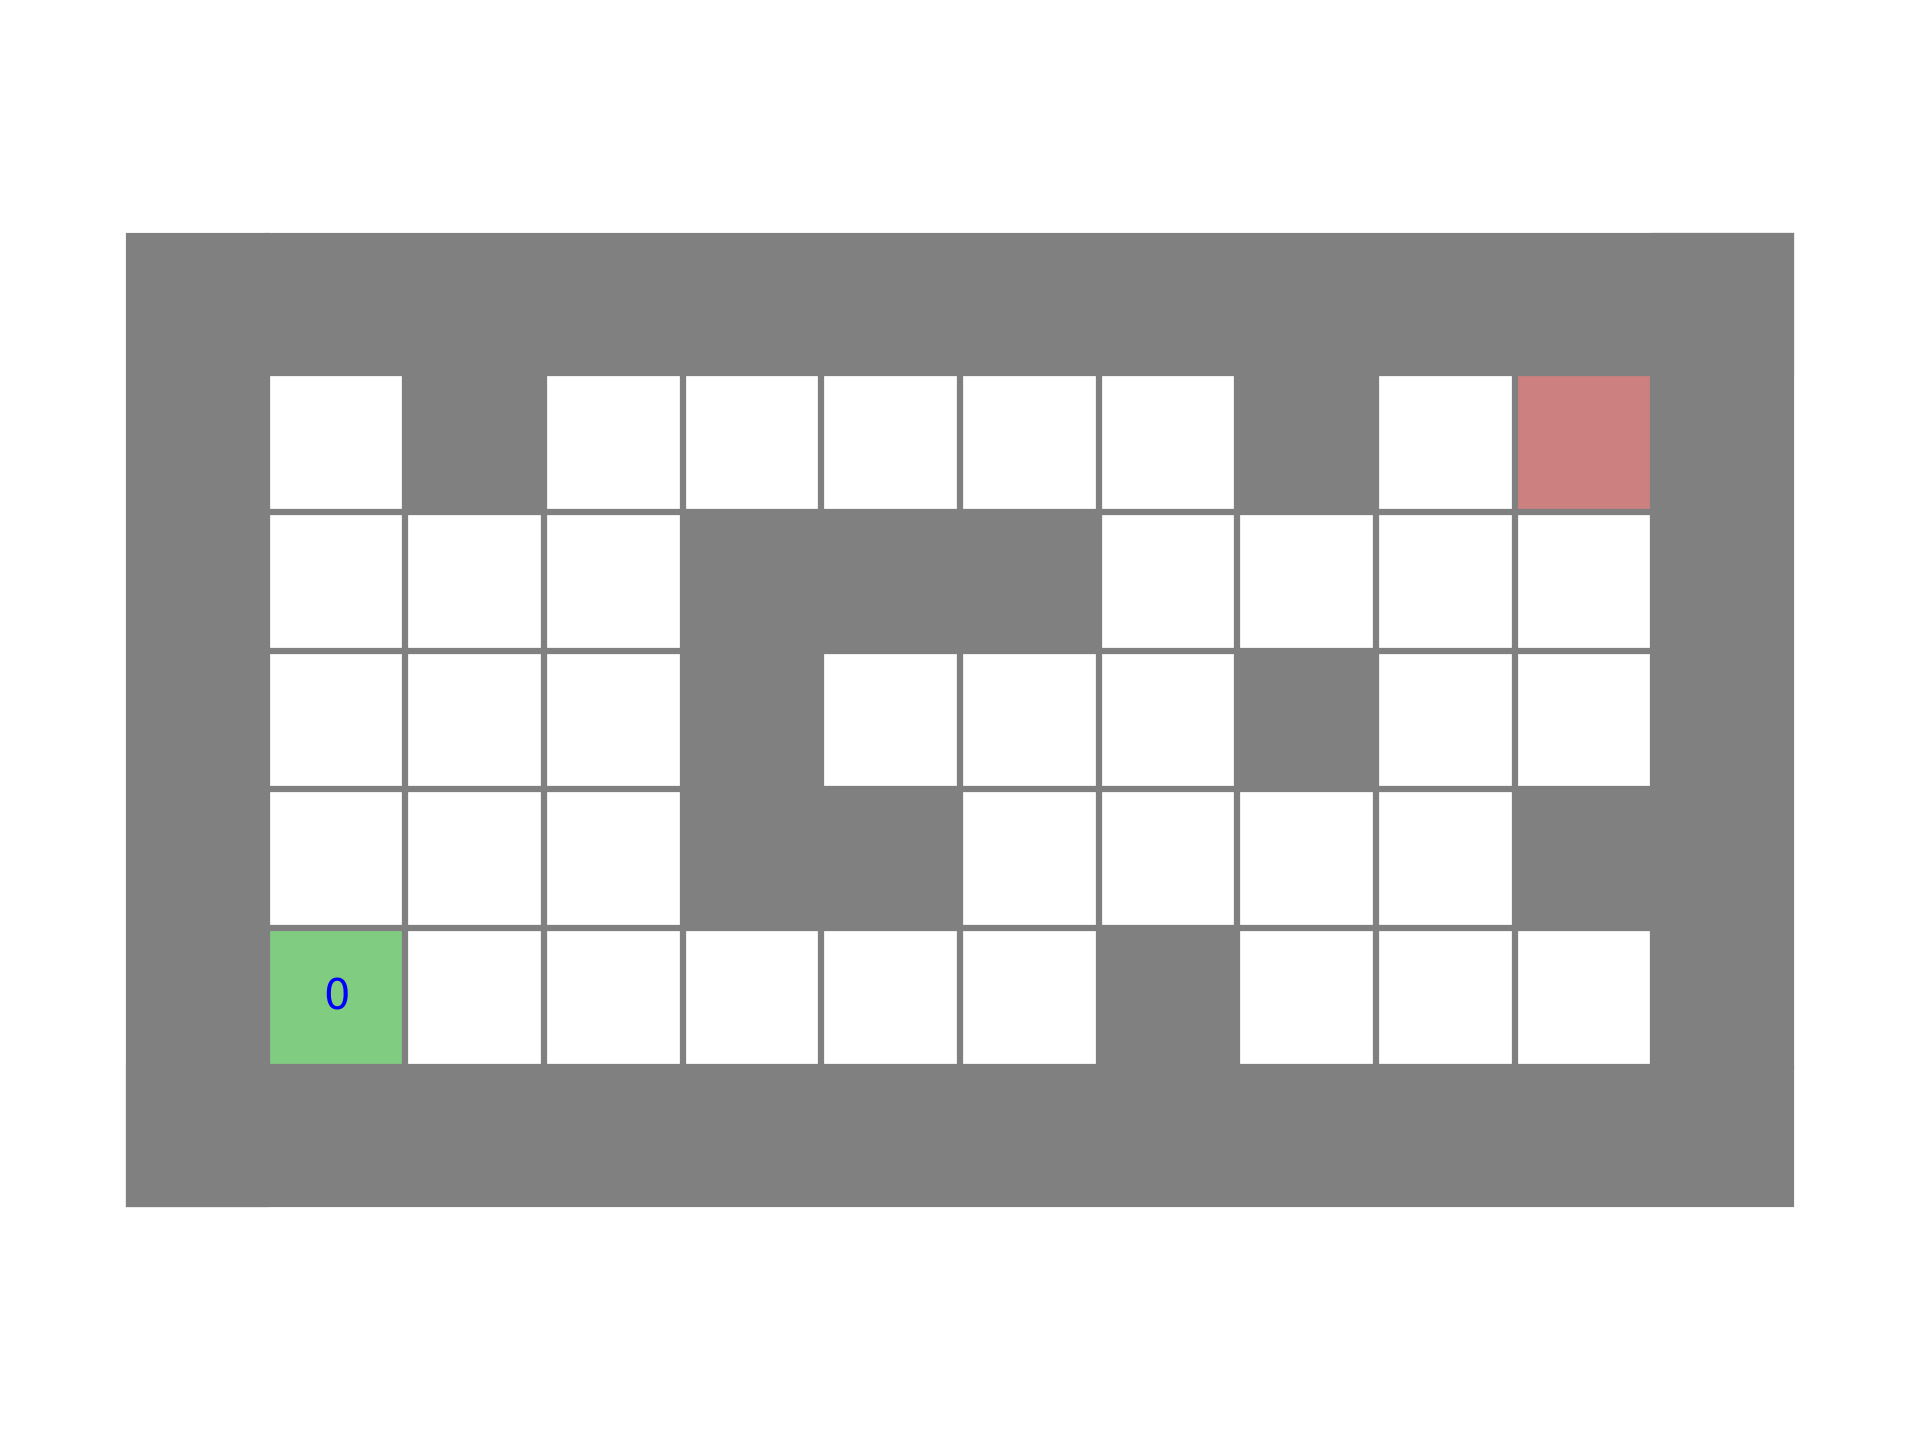
\includegraphics[scale=\myscale,scale=0.33]{figures/labyrinthe-01-0}
	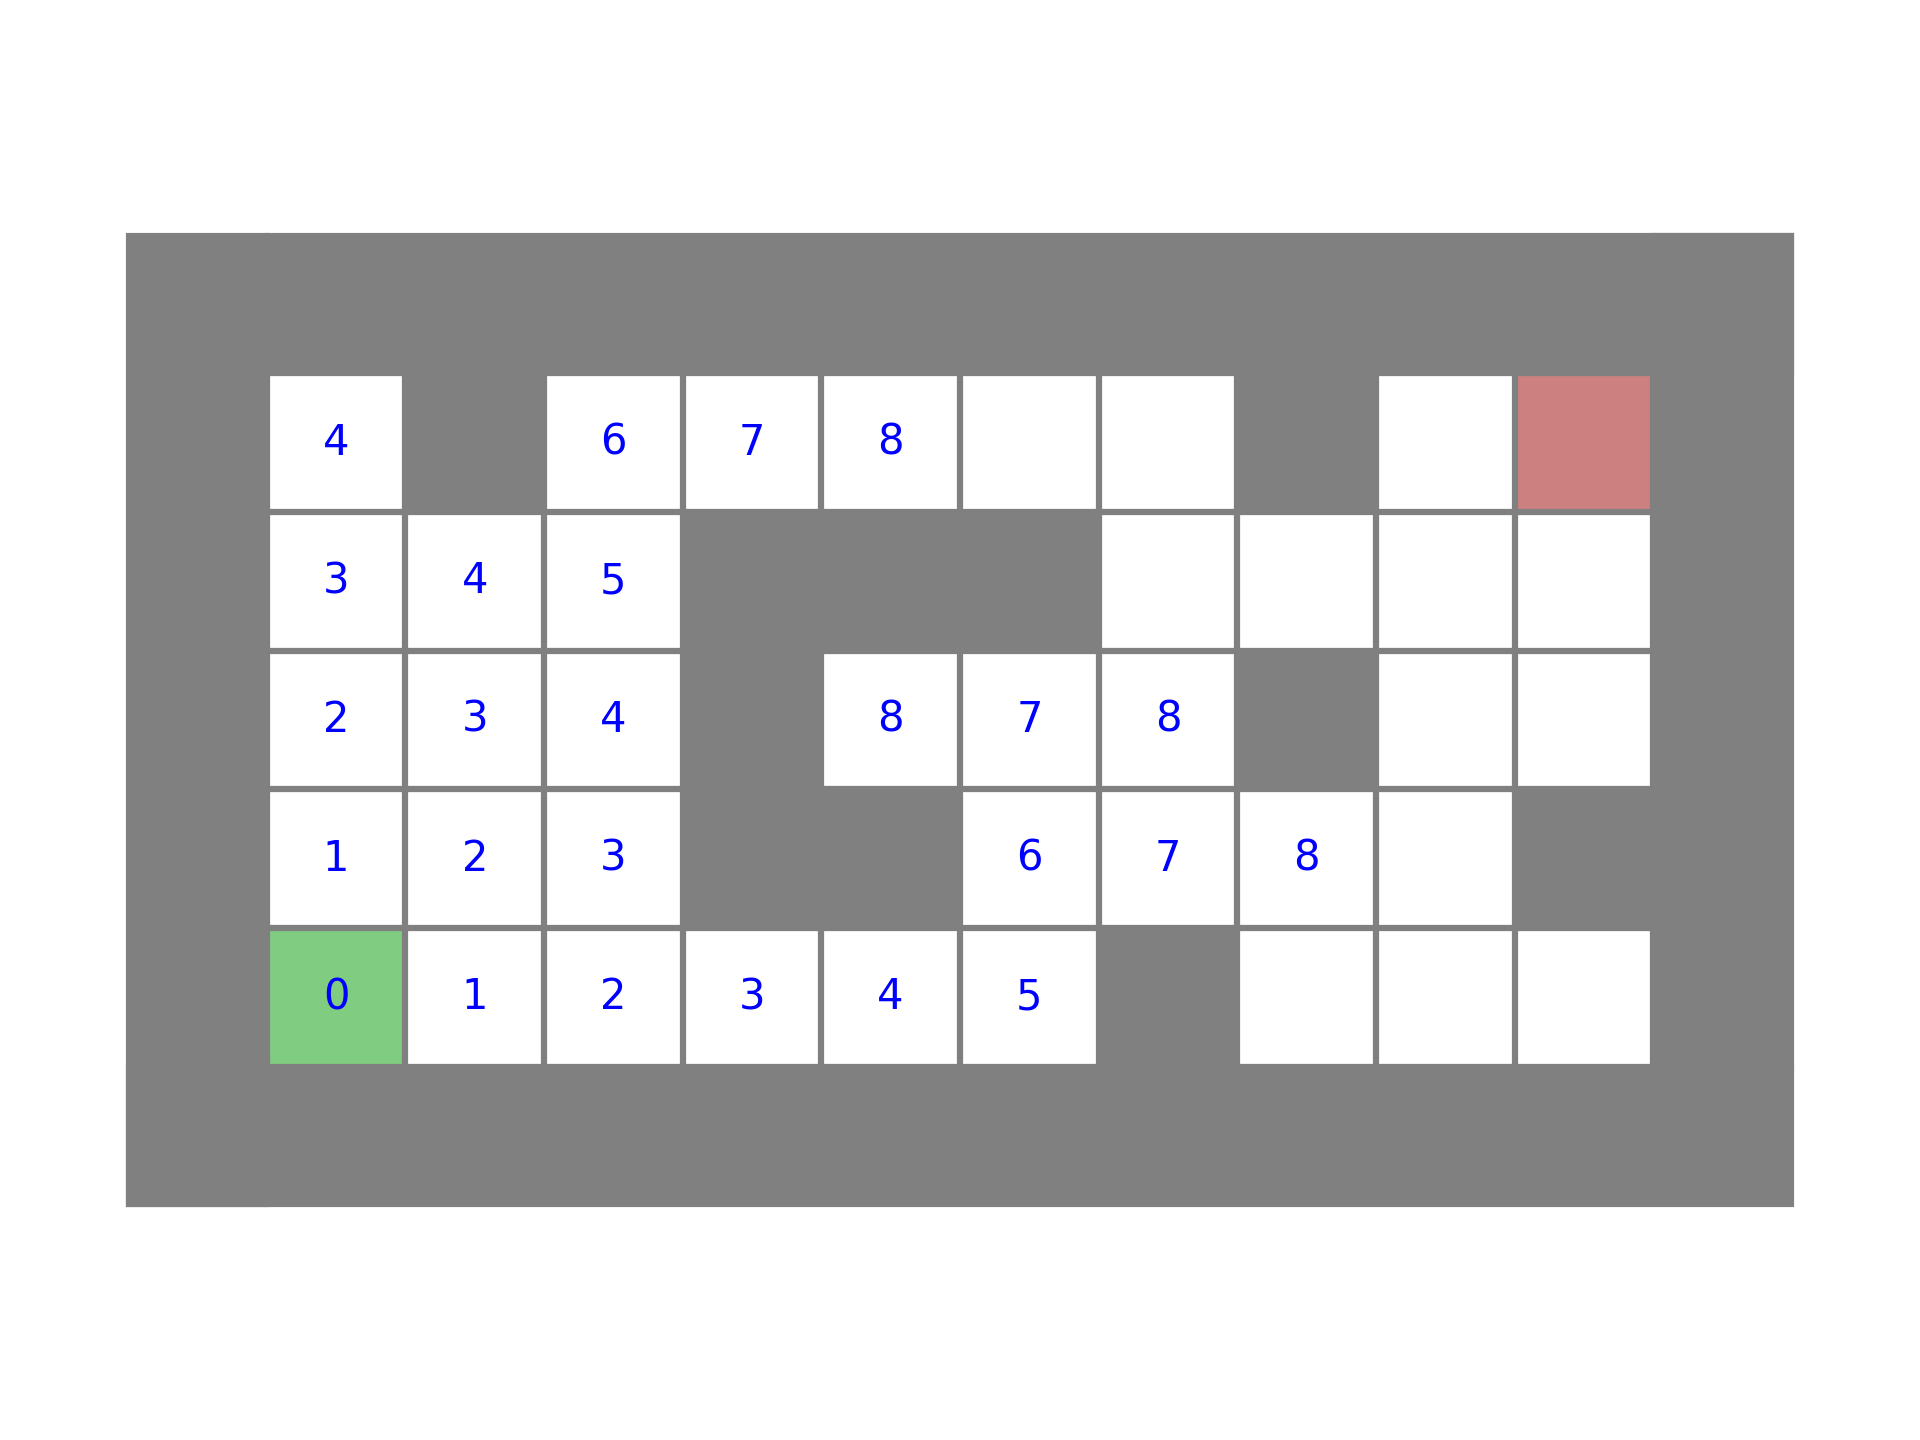
\includegraphics[scale=\myscale,scale=0.33]{figures/labyrinthe-01-8}
	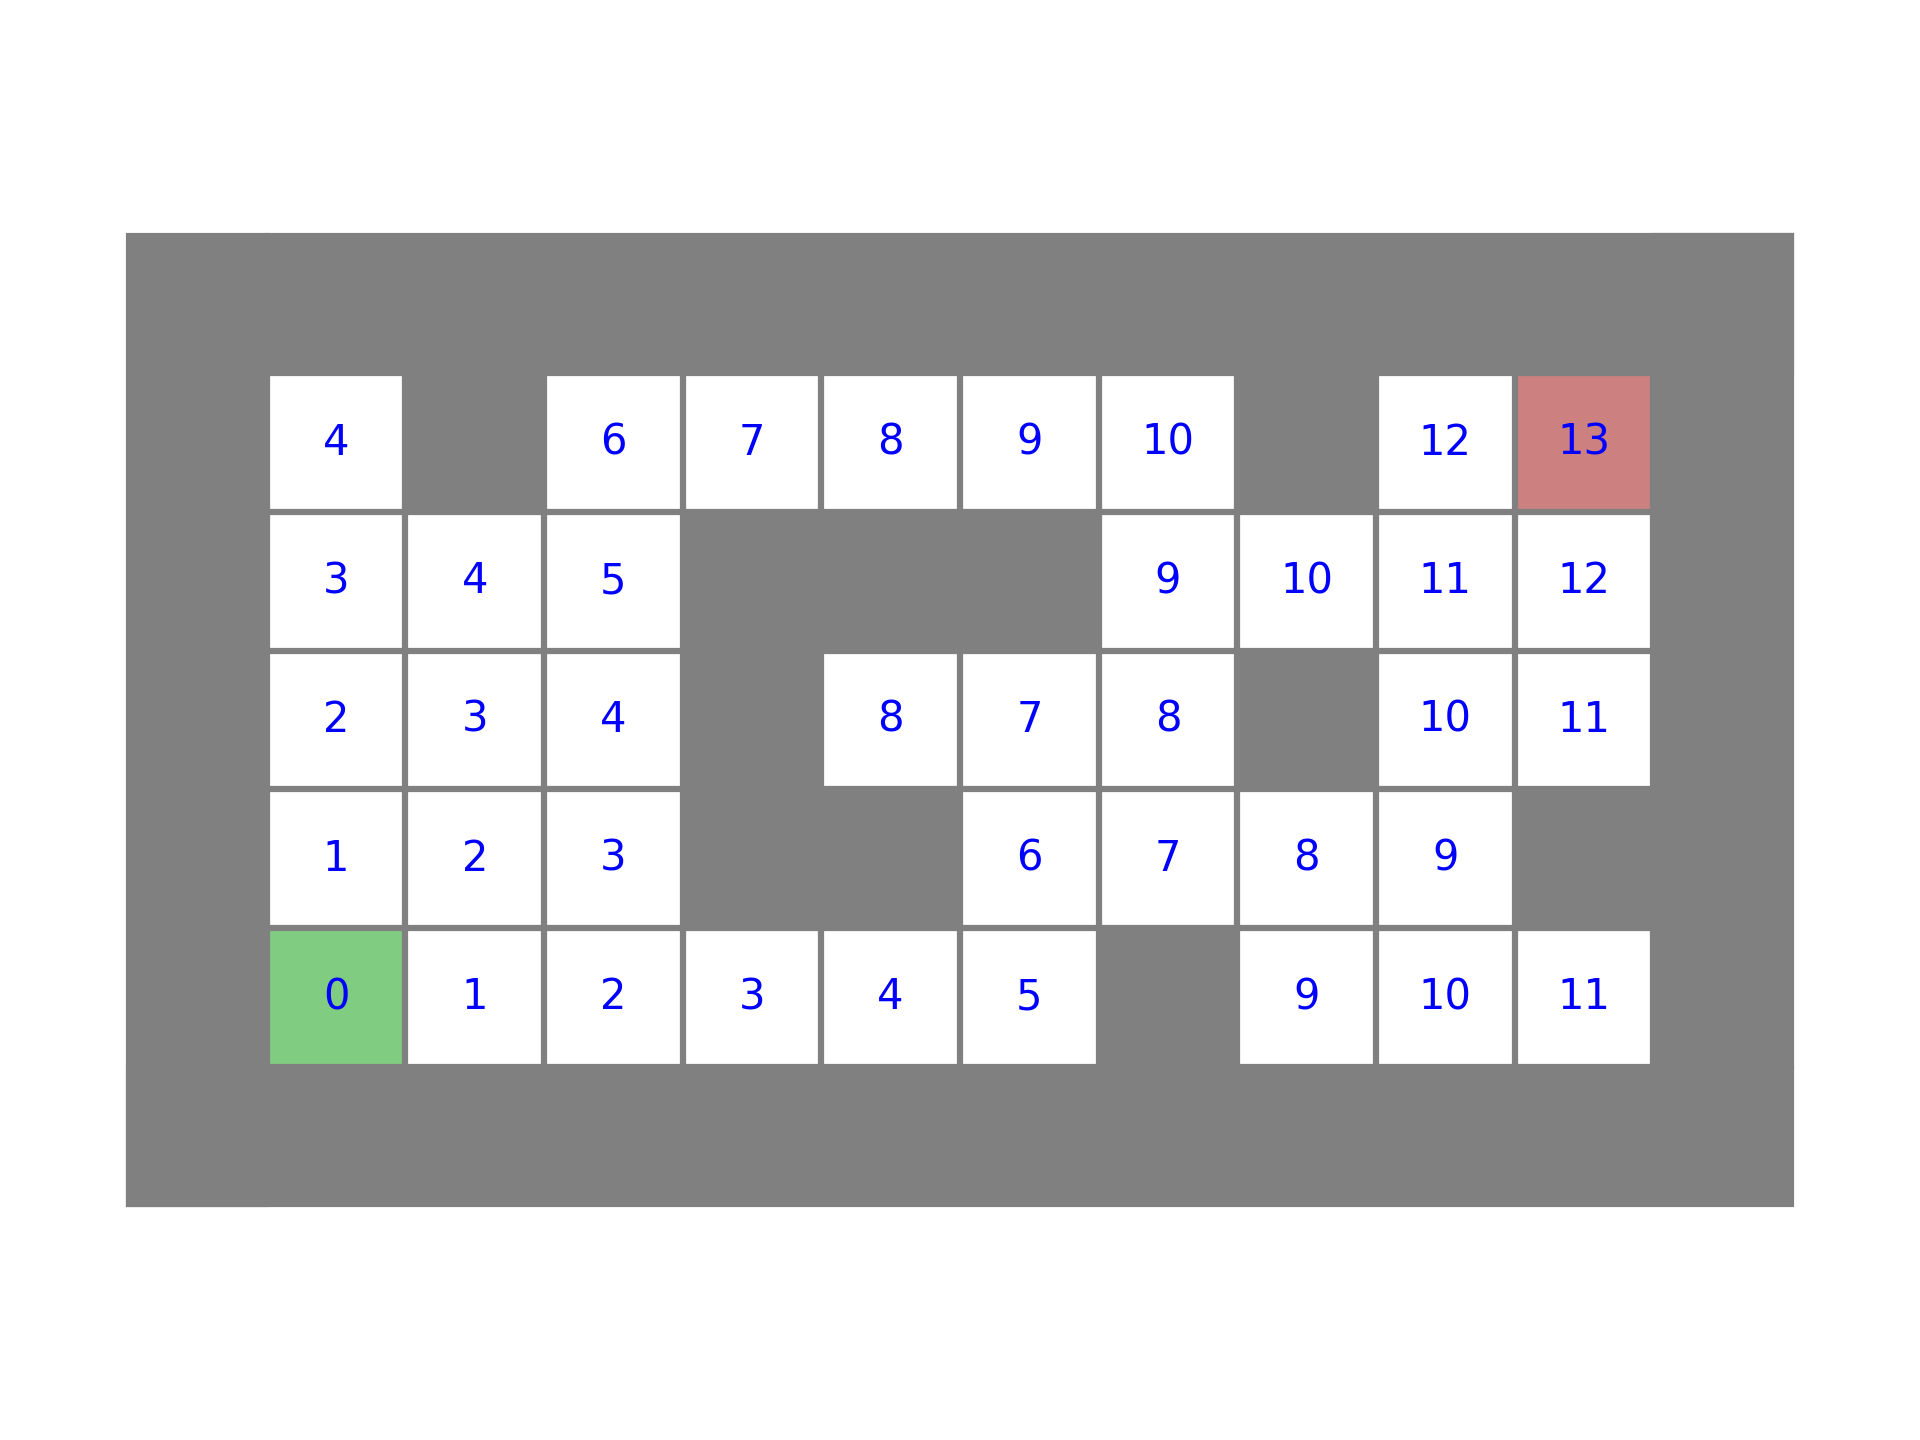
\includegraphics[scale=\myscale,scale=0.33]{figures/labyrinthe-01-13}
\end{center}

Pour obtenir un chemin et la distance reliant le départ et l'arrivée il suffit de partir de la fin et de chercher à chaque étape un voisin strictement plus proche du départ.

\myfigure{0.6}{
	\tikzinput{fig-labyrinthe-09}	
}


\begin{algorithme}[Chemin reliant le départ et l'arrivée]
Entrée : un graphe, un sommet \og{}départ\fg{}, un sommet \og{}arrivée\fg{} et pour chaque sommet du graphe sa distance au sommet \og{}départ\fg{}.

Sortie  : un chemin reliant le départ à l'arrivée.

\begin{itemize}
	\item Se placer au sommet $s$ de l'arrivée, initialiser une liste \ci{chemin} à $s$.
	
	\item Tant que $s$ n'est pas le sommet de départ :
	\begin{itemize}
		\item parmi les voisins de $s$, choisir $s'$ tel que $d(s') < d(s)$,
		\item ajouter $s'$ à \ci{chemin},
		\item faire $s \leftarrow s'$.
	\end{itemize}	
\end{itemize}  
\end{algorithme}

Lors du choix de $s'$ parmi les voisins de $s$ vérifiant $d(s') < d(s)$ il y a (par construction) au moins une possibilité, s'il y en a plusieurs, on peut  choisir n'importe laquelle (au hasard par exemple).

\begin{center}
	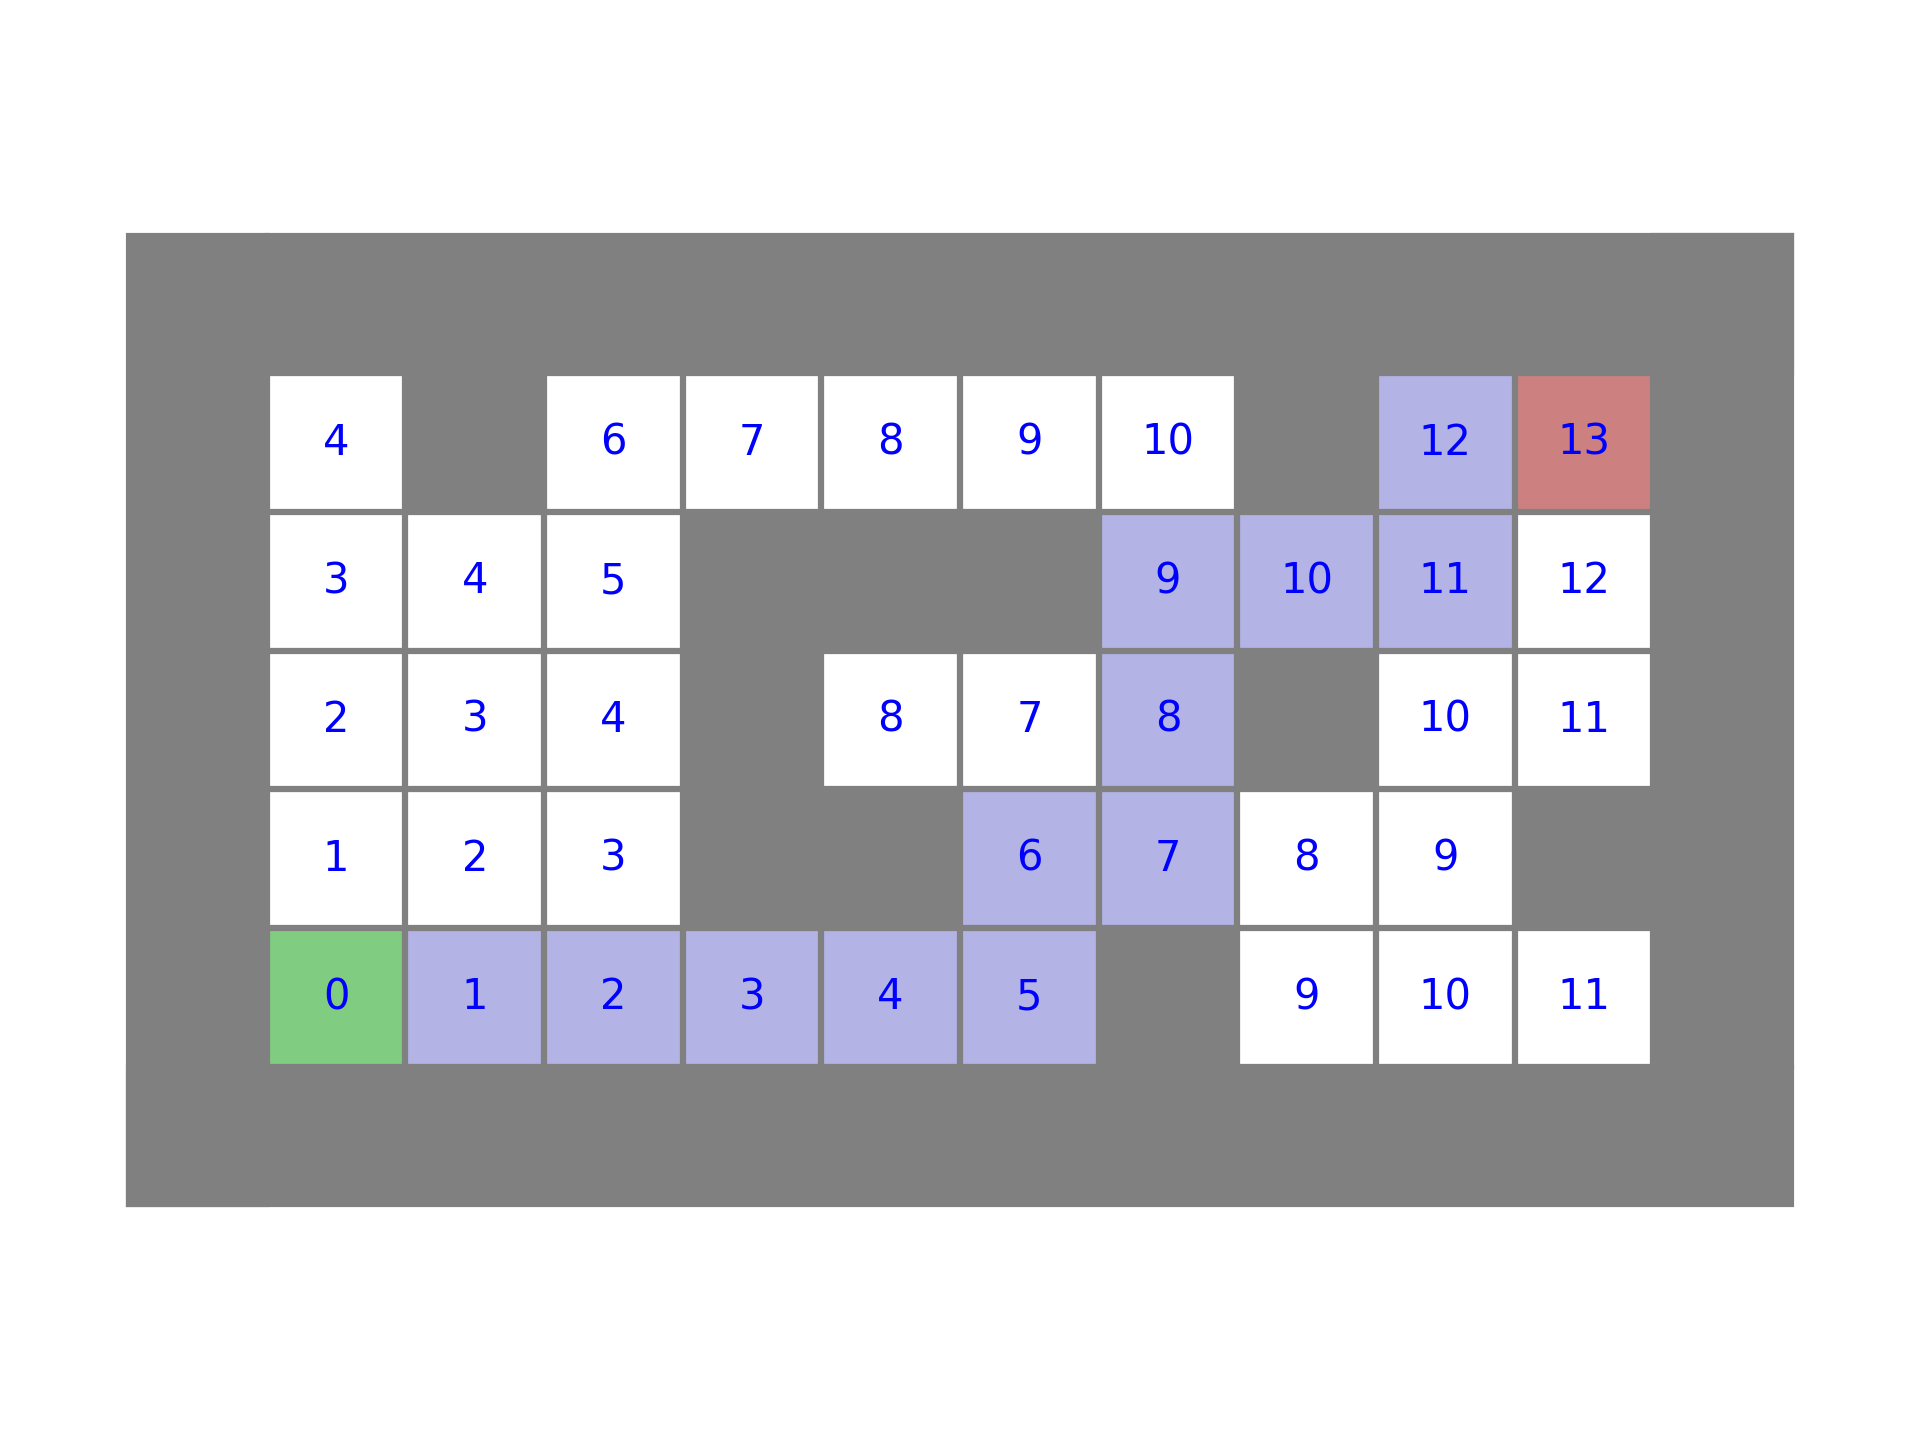
\includegraphics[scale=\myscale,scale=0.43]{figures/labyrinthe-01-14}
	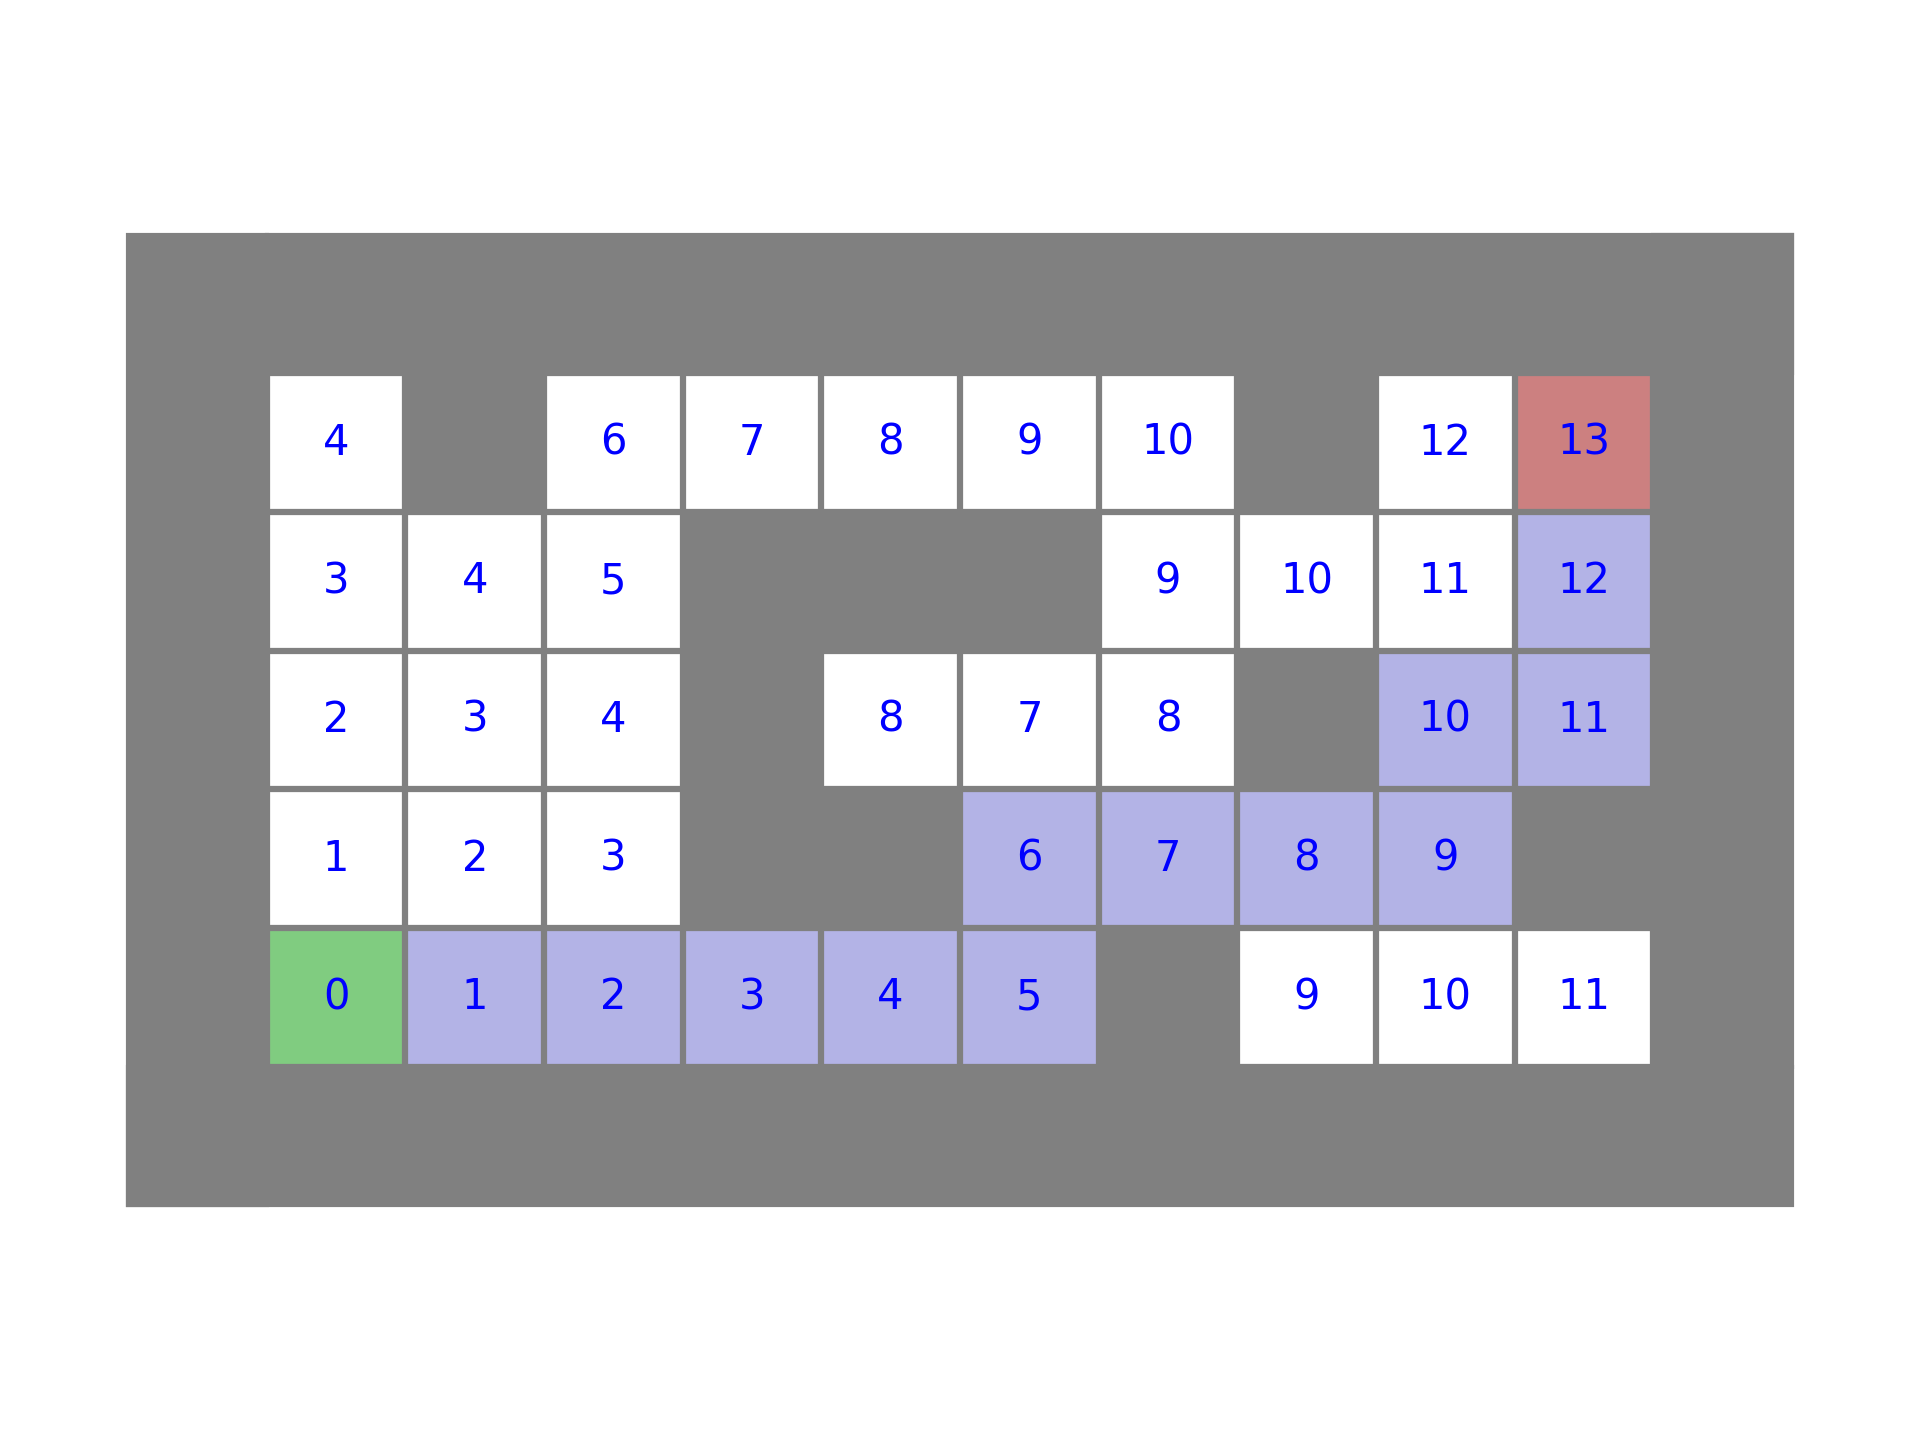
\includegraphics[scale=\myscale,scale=0.43]{figures/labyrinthe-01-15}
\end{center}


\begin{center}
	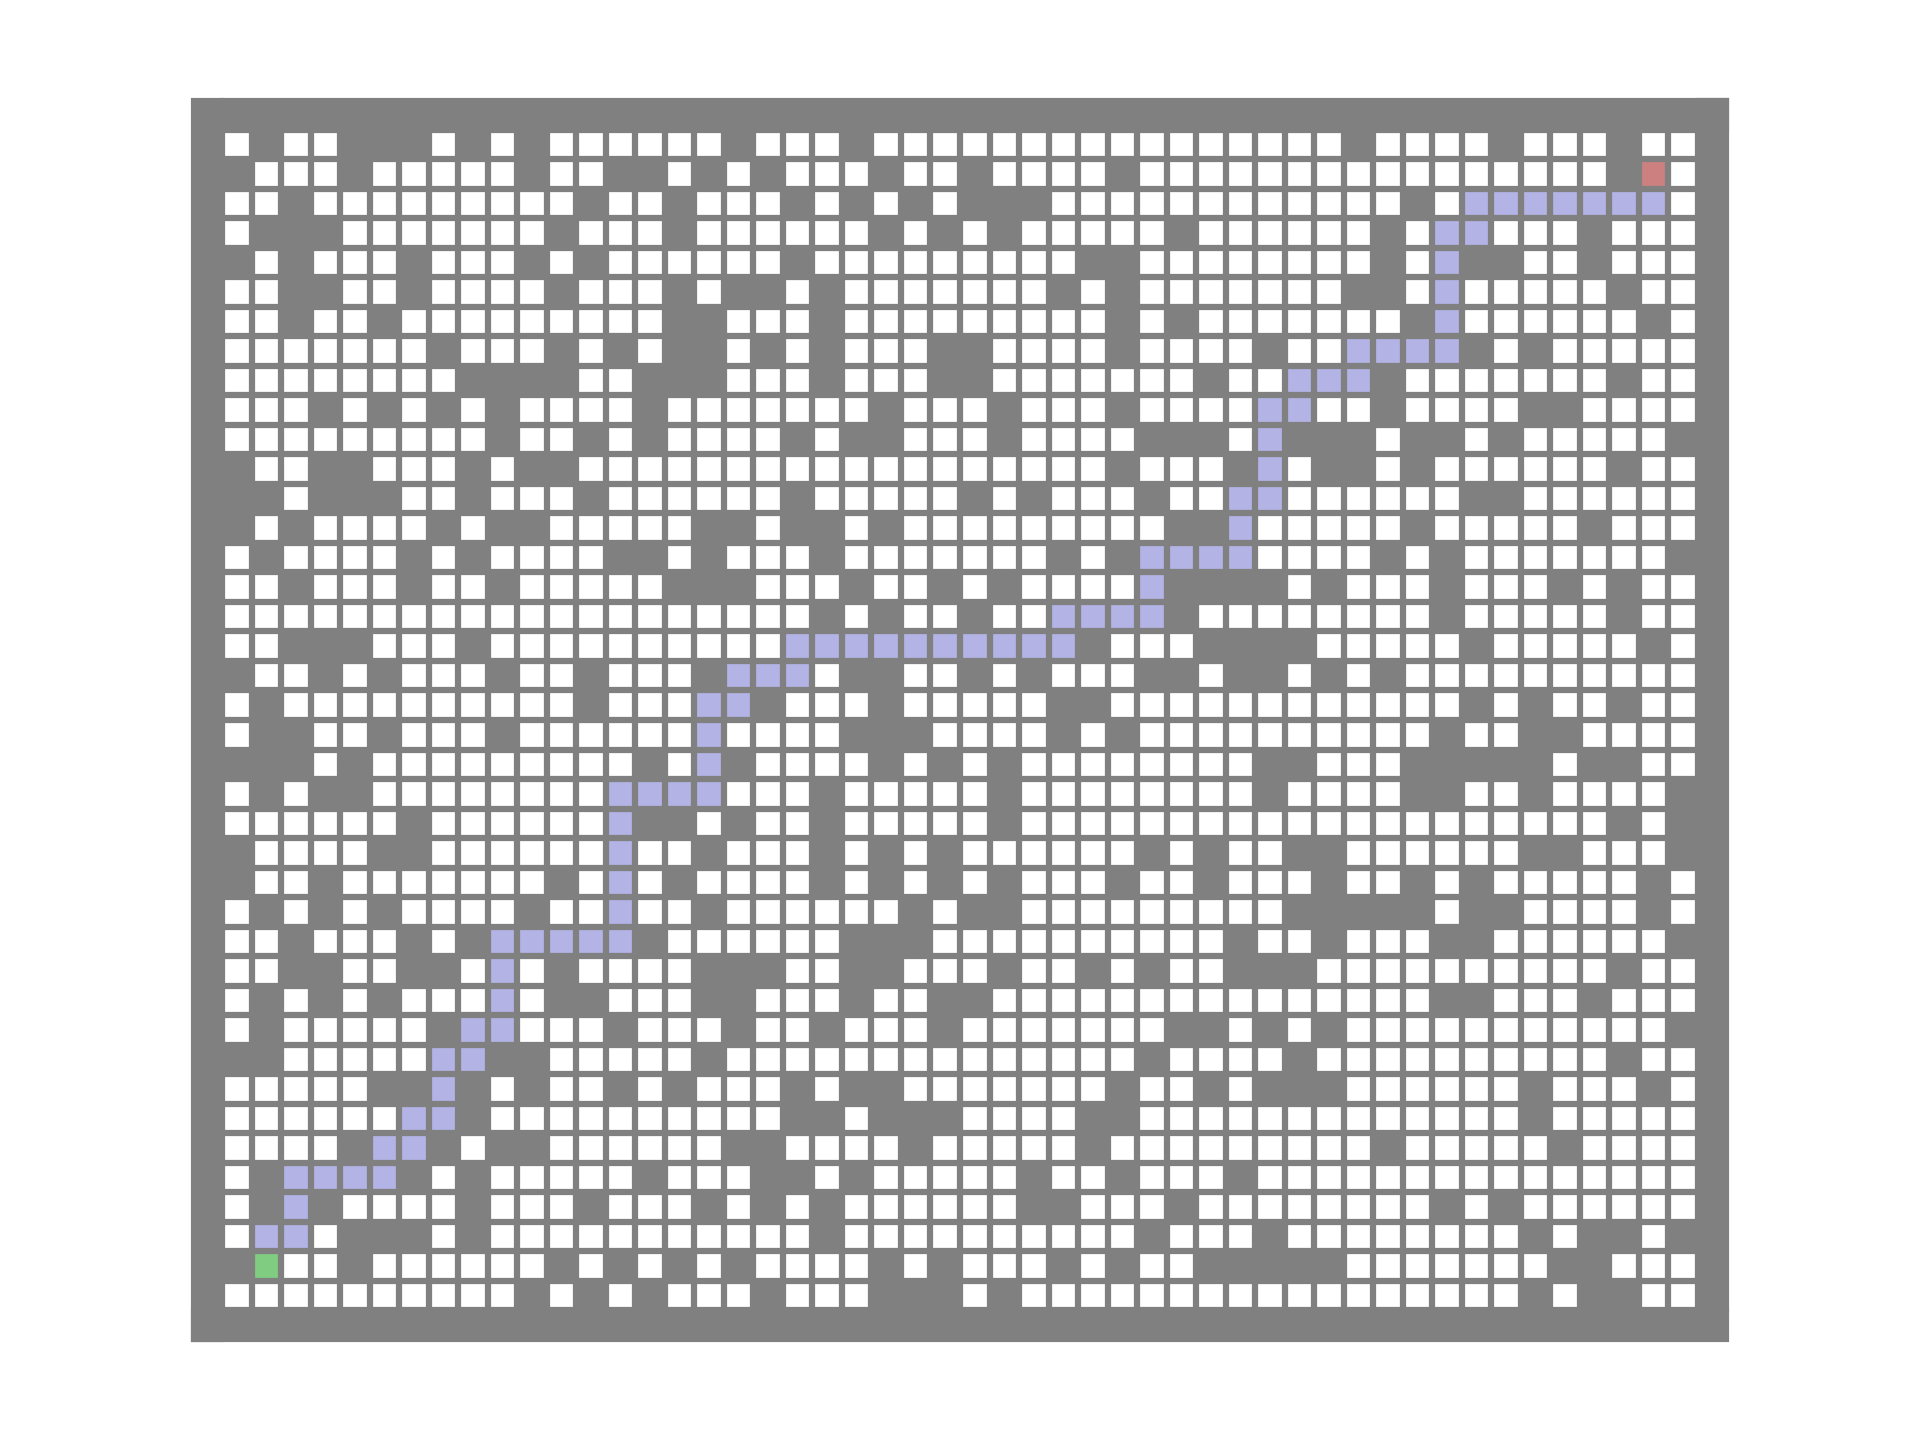
\includegraphics[scale=\myscale,scale=0.5]{figures/labyrinthe-02-1}
	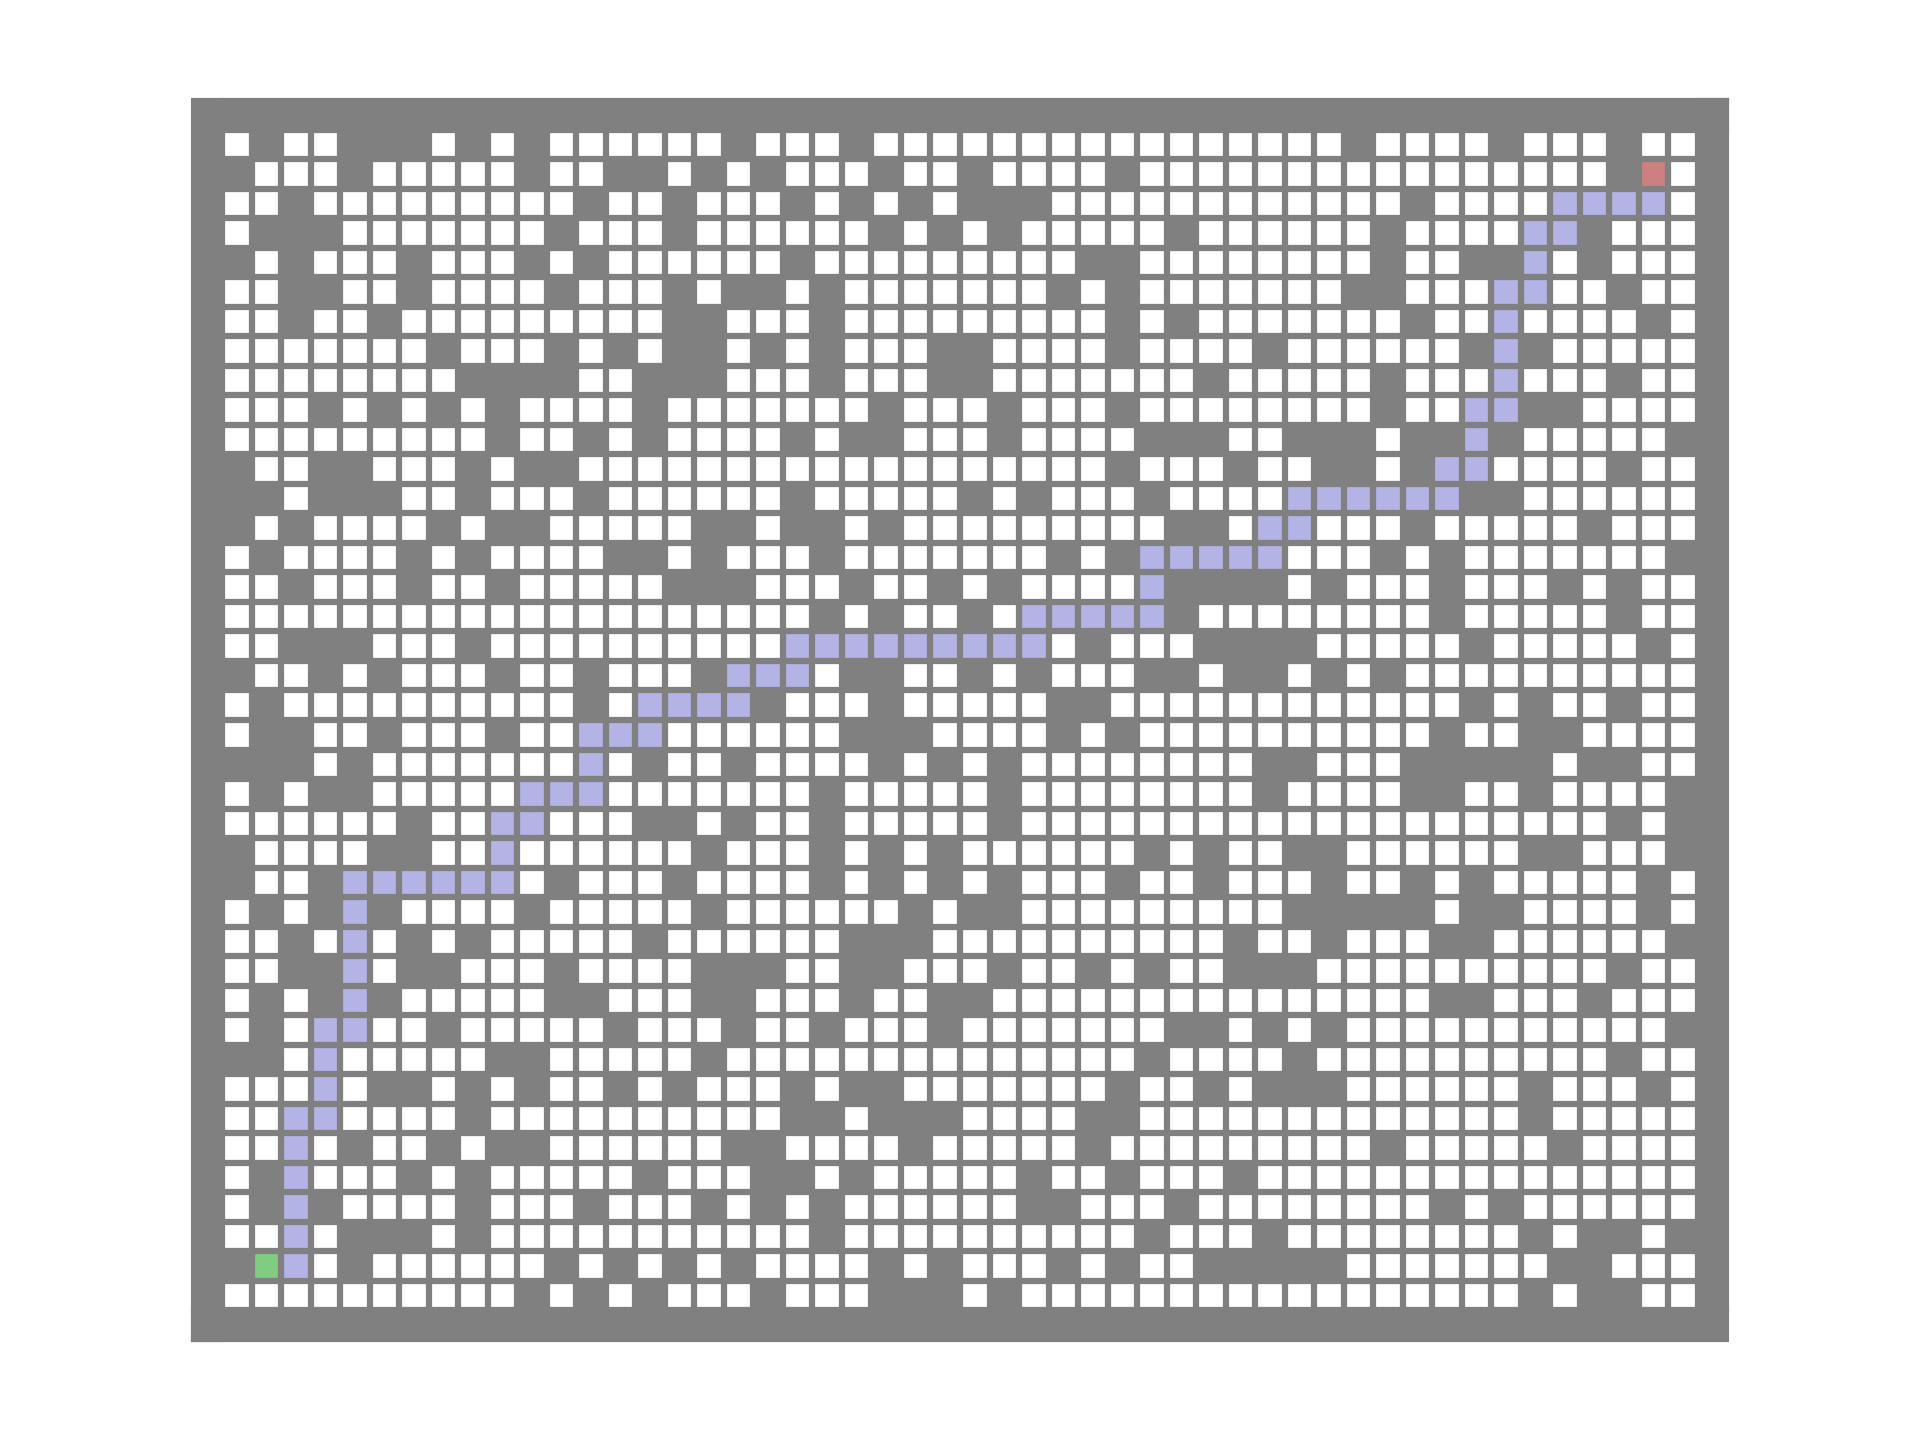
\includegraphics[scale=\myscale,scale=0.5]{figures/labyrinthe-02-2}
\end{center}


%%%%%%%%%%%%%%%%%%%%%%%%%%%%%%%%%%%%%%%%%%%%%%%%%%%%%%%%%%%%%%%%%%%%%
\section{Terrain}

%--------------------------------------------------------------------
\subsection{Modélisation}

Un personnage à la position $P$ doit atteindre l'objectif $X$.
Si le terrain est dégagé alors il se déplace en ligne droite en direction de l'objectif. S'il avance d'un pas de longueur $\delta$ alors sa nouvelle position est :
$$P' = P + \delta \frac{\vec{PX}}{\| \vec{PX} \|}.$$

\myfigure{0.6}{
	\tikzinput{fig-terrain-01}	
}

Mais comment se déplacer s'il y a des obstacles sur son trajet ? 
Et si le terrain n'est pas uniforme, par exemple avec des zones où l'avancement est plus difficile : faut-il mieux foncer tout droit ou contourner les difficultés ?

Pour répondre à ces questions, nous allons modéliser un terrain par une grille rectangulaire. Chaque case peut avoir un type de terrain différent.
À chaque type de terrain on attribue une valeur. Plus la valeur est élevée, plus le terrain est difficile et donc la progression plus lente.
Voici les types de terrain qu'on va rencontrer :
\begin{itemize}
	\item terrain facile : valeur $1$,
	\item terrain difficile : valeur $2$ (on s'y déplace deux fois moins vite),
	\item eau/lac : valeur $5$ (on peut nager, mais c'est lent),
	\item obstacle infranchissable : valeur infinie (dans la pratique il suffit de mettre une valeur élevée).
\end{itemize}


\myfigure{0.5}{
	\footnotesize
	\tikzinput{fig-terrain-02}\qquad\qquad	
	\tikzinput{fig-terrain-03}	
}
Dans cette modélisation on autorise les déplacements en diagonale.

%--------------------------------------------------------------------
\subsection{Distances}

Il y a plusieurs façons de mesurer la distance entre deux points.
Ce choix est important.

\myfigure{0.8}{
	\tikzinput{fig-terrain-05}	
}


\textbf{Distance de Manhattan.}
La \defi{norme $1$} est définie par $\| (x,y) \|_1 = |x| + |y|$.
La distance associée s'appelle la distance de Manhattan :
$d_1(A,B) = \| B - A \|_1 = |x_B-x_A| + |y_B-y_A|$,
car elle correspond à la distance qu'il faut parcourir lorsqu'on se déplace sur une grille.

Pour une case, ses voisins immédiats sont donc les $4$ cases situées immédiatement à gauche/droite/haut/bas, les centres des cases placées en diagonale sont à une distance $2$ du centre de la case centrale.


\myfigure{0.7}{
	\tikzinput{fig-terrain-04}	
}


\bigskip

\textbf{Distance euclidienne.}
La \defi{norme $2$} est définie par $\| (x,y) \|_2 = \sqrt{ x^2 + y^2}$.
La distance associée s'appelle la distance euclidienne :
$d_2(A,B) = \| B - A \|_2 = \sqrt{ (x_B-x_A)^2 + (y_B-y_A)^2}$,
c'est la distance usuelle \og{}à vol d'oiseau\fg{}.
Cette fois les centres des cases en diagonale sont à une distance $\sqrt2$ du centre de la case centrale.


\bigskip

\textbf{Distance de Tchebychev.}
La \defi{norme infinie} est définie par $\| (x,y) \|_\infty = \max( |x|, |y| )$.
La distance associée s'appelle la distance de Tchebychev :
$d_\infty(A,B) = \| B - A \|_{\infty} = \max( |x_B-x_A|, |y_B-y_A|)$.
Avec cette distance, les cases en diagonale sont des voisins immédiats de la case centrale.


%--------------------------------------------------------------------
\subsection{Heatmap}

On fixe l'une des distances précédentes.
Pour se diriger on commence par calculer une \emph{heatmap}, c'est-à-dire une carte de chaleur. Plus une case est rouge plus elle est proche de l'objectif, les teintes bleues correspondent aux cases plus éloignées.

Ci-dessous, de gauche à droite : (a) le terrain, (b) la distance à la case d'arrivée (selon la distance de Manhattan), (c) les couleurs de la \emph{heatmap}.

\begin{center}
	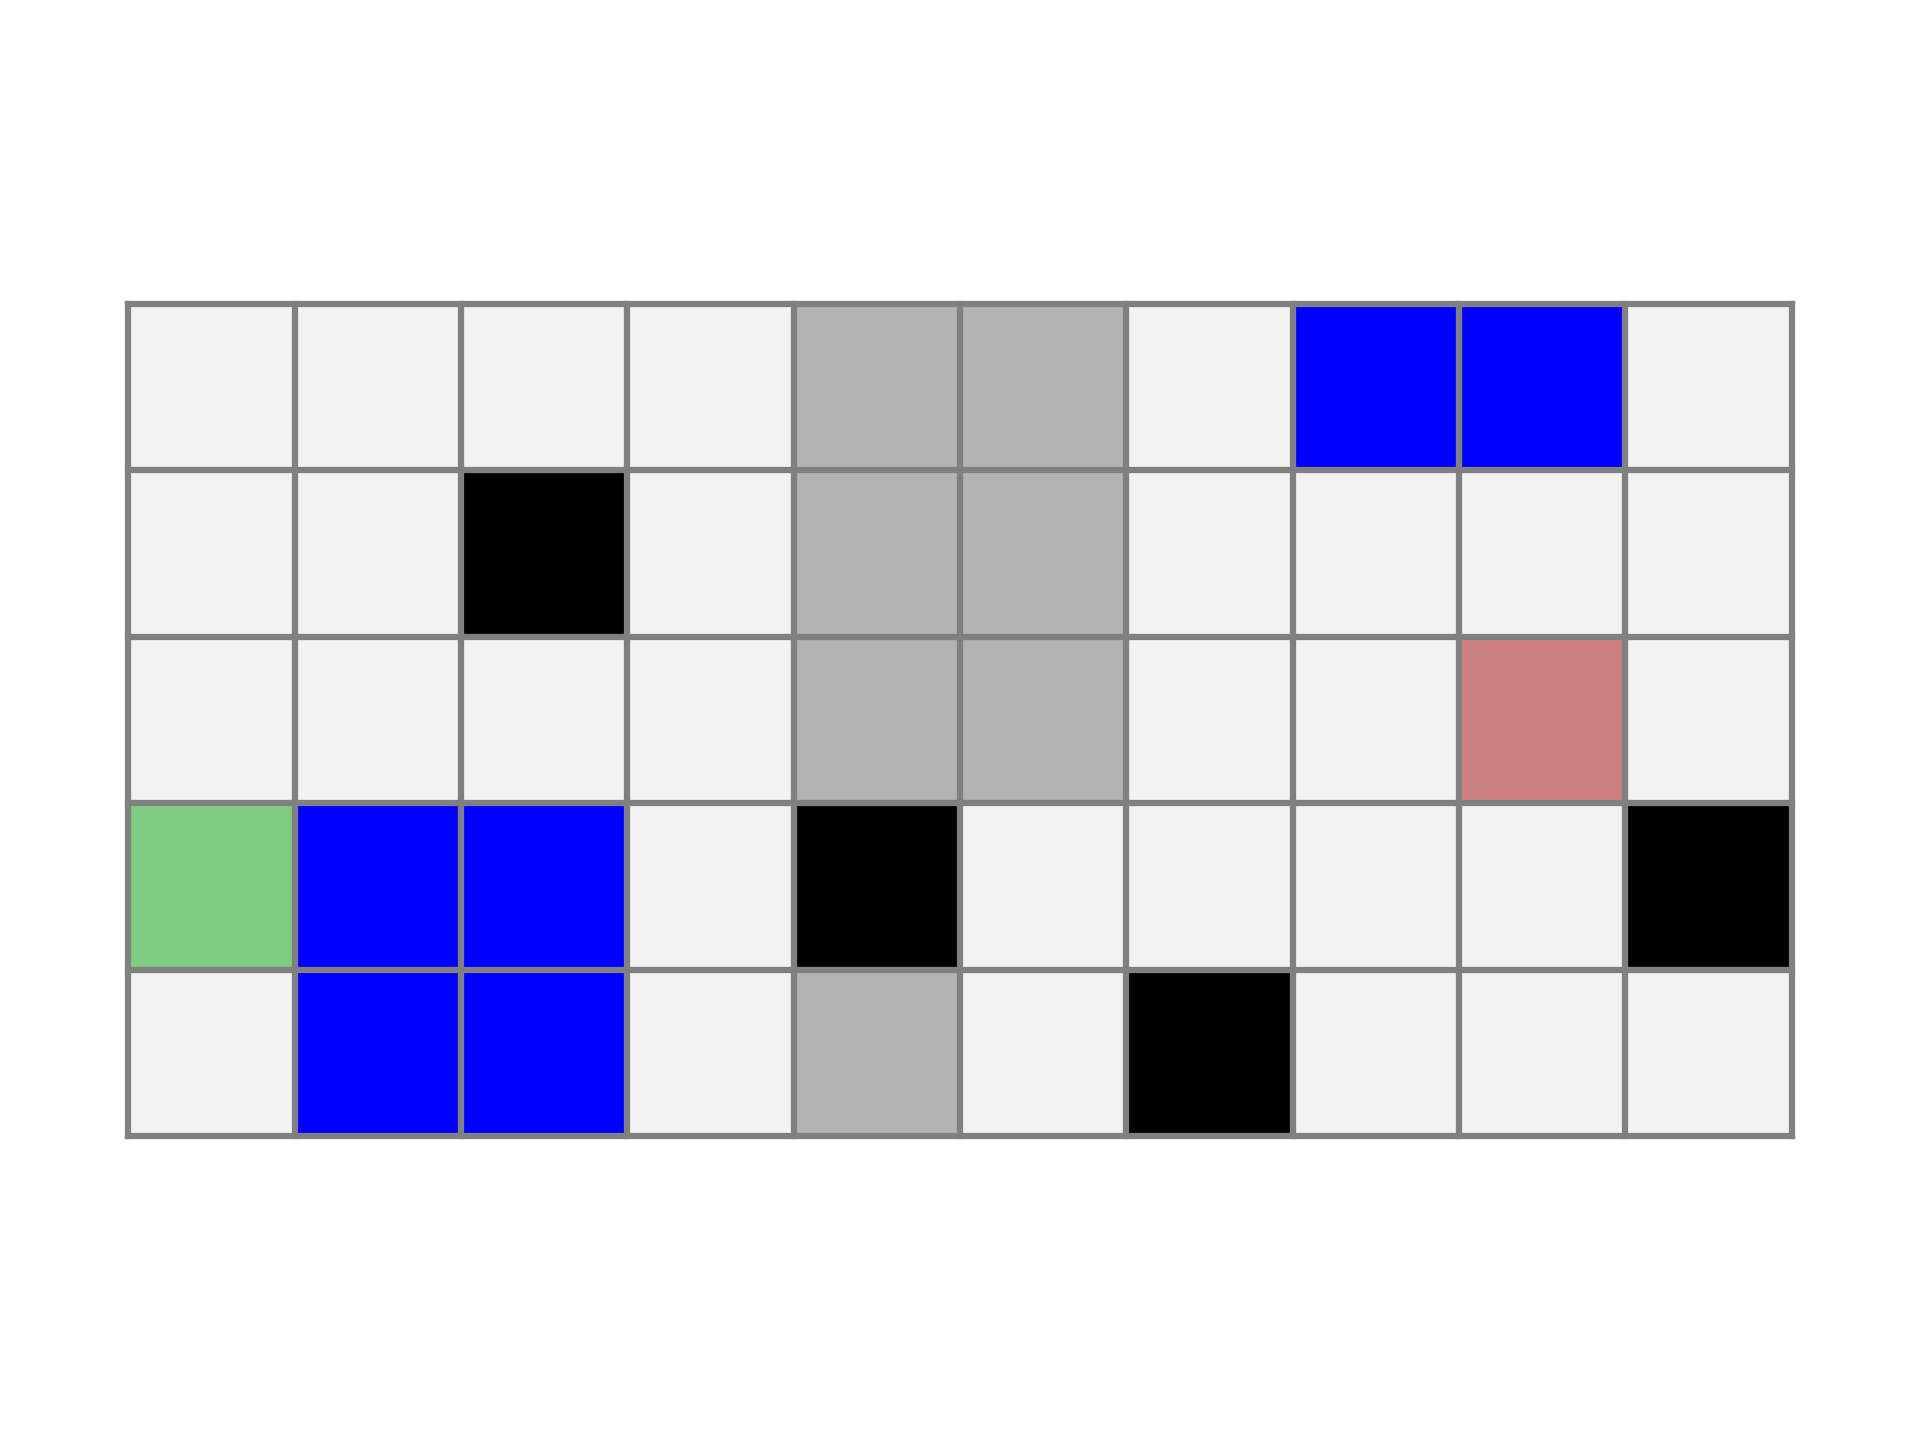
\includegraphics[scale=\myscale,scale=0.33,trim={0 2cm 0 2cm},clip]{figures/terrain-01-1}
	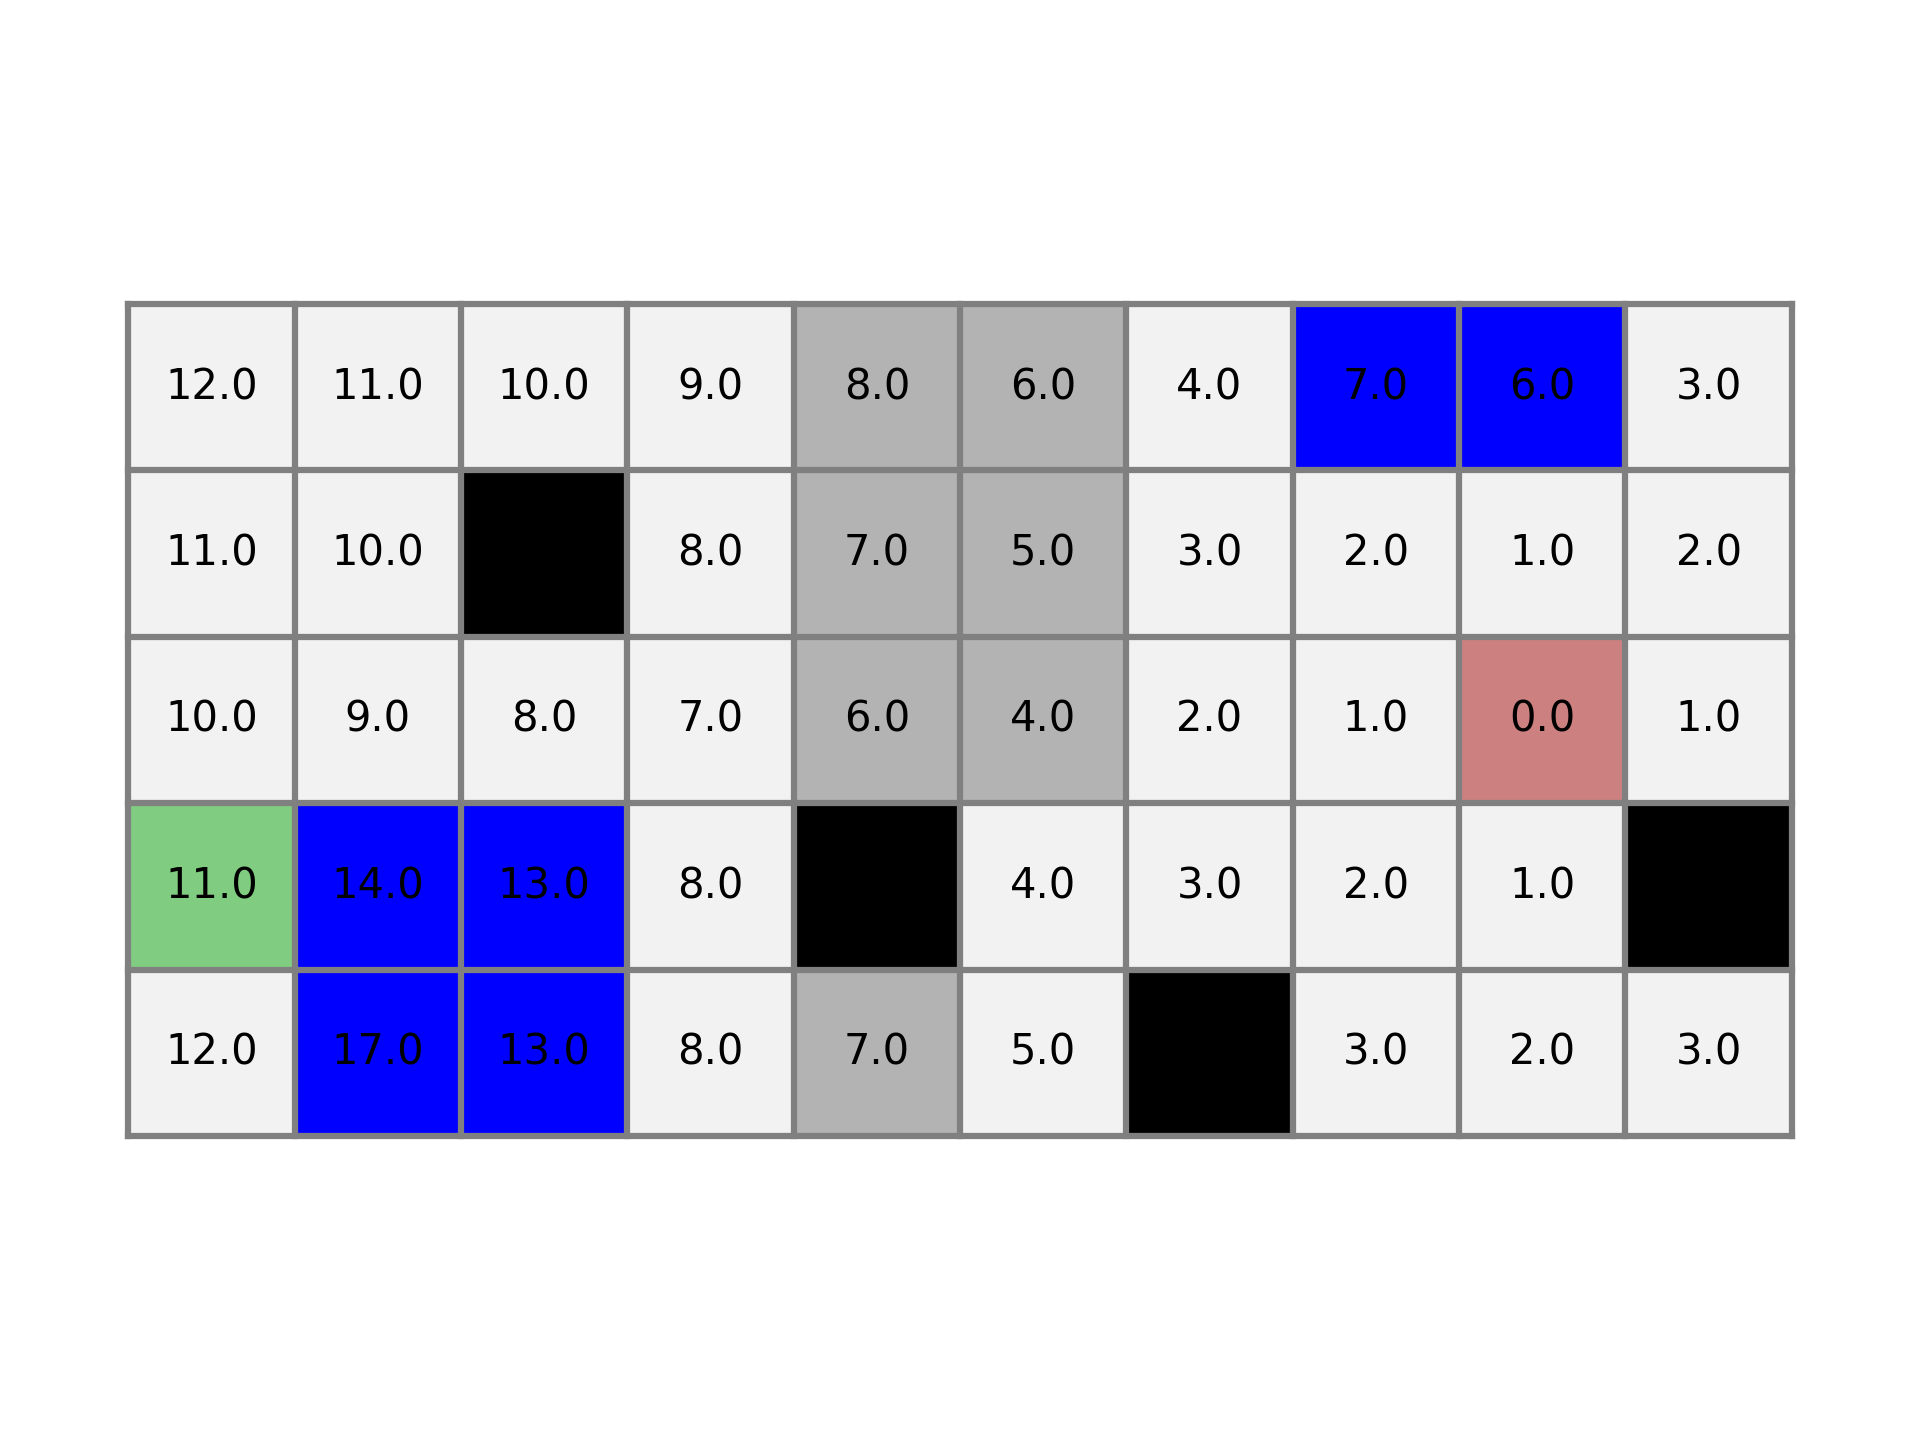
\includegraphics[scale=\myscale,scale=0.33,trim={0 2cm 0 2cm},clip]{figures/terrain-01-2}
	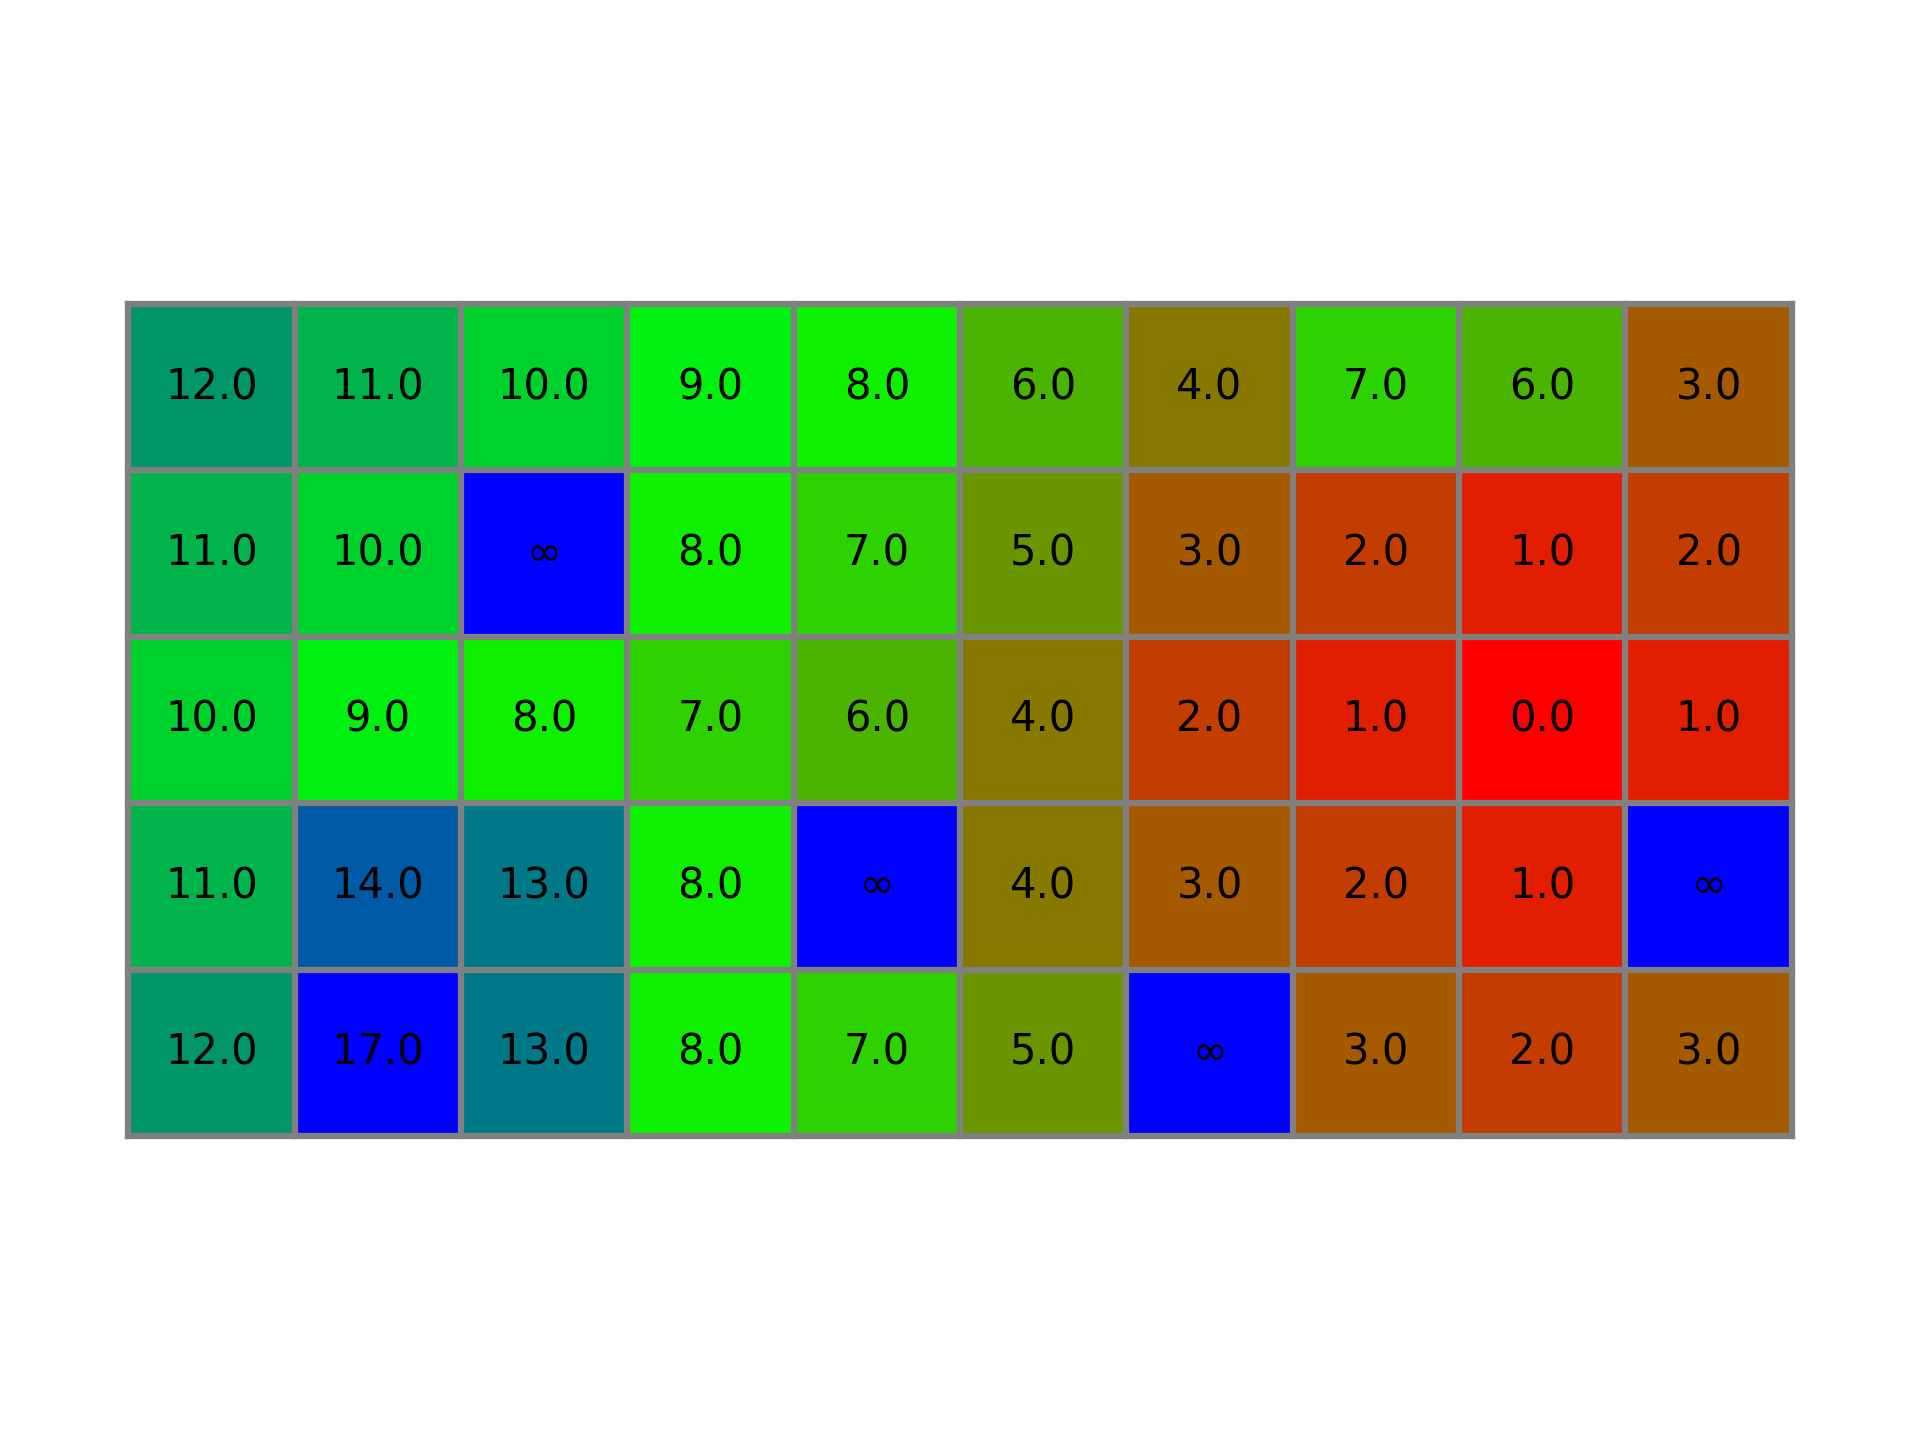
\includegraphics[scale=\myscale,scale=0.33,trim={0 2cm 0 2cm},clip]{figures/terrain-01-3}
\end{center}


Concrètement la \emph{heatmap} est une fonction $h$ qui à chaque case $(i,j)$ lui associe sa distance à l'objectif.
Si on passe par une case de valeur $1$, la distance augmente de $1$, si on passe sur un terrain plus difficile, par exemple une case d'eau, la distance augmente de $5$. On tient compte en plus de la distance entre deux cases voisines (qui n'est pas toujours $1$ pour les cases en diagonales).

L'algorithme du calcul de la \emph{heatmap} est similaire au calcul de la distance utilisé pour les labyrinthes mais il y a un subtilité supplémentaire car les distances associées à chaque case dépendent du terrain.

Ci-dessous on commence par compléter les distances case par case. On commence par la case d'arrivée (en rouge, figure (b)) qui a pour valeur de la \emph{heatmap} $0$. On atteint assez vite la case de départ (en vert, figure (c)), mais lorsqu'on continue de compléter les distances on s'aperçoit qu'il existe un chemin plus rapide même si on parcourt plus de cases (figures (d) et (e)) et cela oblige à mettre à jour la distance entre la case de départ et celle d'arrivée.

\myfigure{0.7}{
	\footnotesize
	\tikzinput{fig-terrain-06}	
}


Comme auparavant on identifie la grille à un graphe: une case correspond à un sommet, les sommets adjacents correspondent aux $8$ cases voisines (y compris les cases en diagonale).



\begin{algorithme}[Calcul de la \emph{heatmap}]

Entrée : un graphe (connexe) avec un sommet \og{}arrivée\fg{}, la valeur $t(s)$ du terrain associée à chaque sommet et le choix d'une distance $d$.

Sortie : pour chaque sommet $s$, la longueur $h(s)$ du plus petit chemin le reliant au départ.

\begin{itemize}
	\item Pour tous les sommets, initialiser $h(s)$ à $+\infty$.
	
	\item Mettre le sommet $s$ d'\og{}arrivée\fg{} dans la file et pour ce sommet poser $h(s) = 0$.
	
	\item Tant que la file n'est pas vide :
	\begin{itemize}
		\item prendre $s$ le premier sommet de la file (et le retirer de la file),
		\item pour chaque voisin $s'$ de $s$ (même ceux déjà visités) :
		\begin{itemize}
			\item calculer $H = h(s) + d(s,s') \times t(s')$
			\item si $H < h(s')$, alors :
		     \begin{itemize}
	              \item poser $h(s') = H$,
	              \item ajouter $s'$ à la fin de la file.
             \end{itemize}			
		\end{itemize}
	\end{itemize}	
	
\end{itemize}  
\end{algorithme}

Ci-dessous, de gauche à droite, les valeurs de la \emph{heatmap} pour les normes $1$, $2$ et infinie.
\begin{center}
	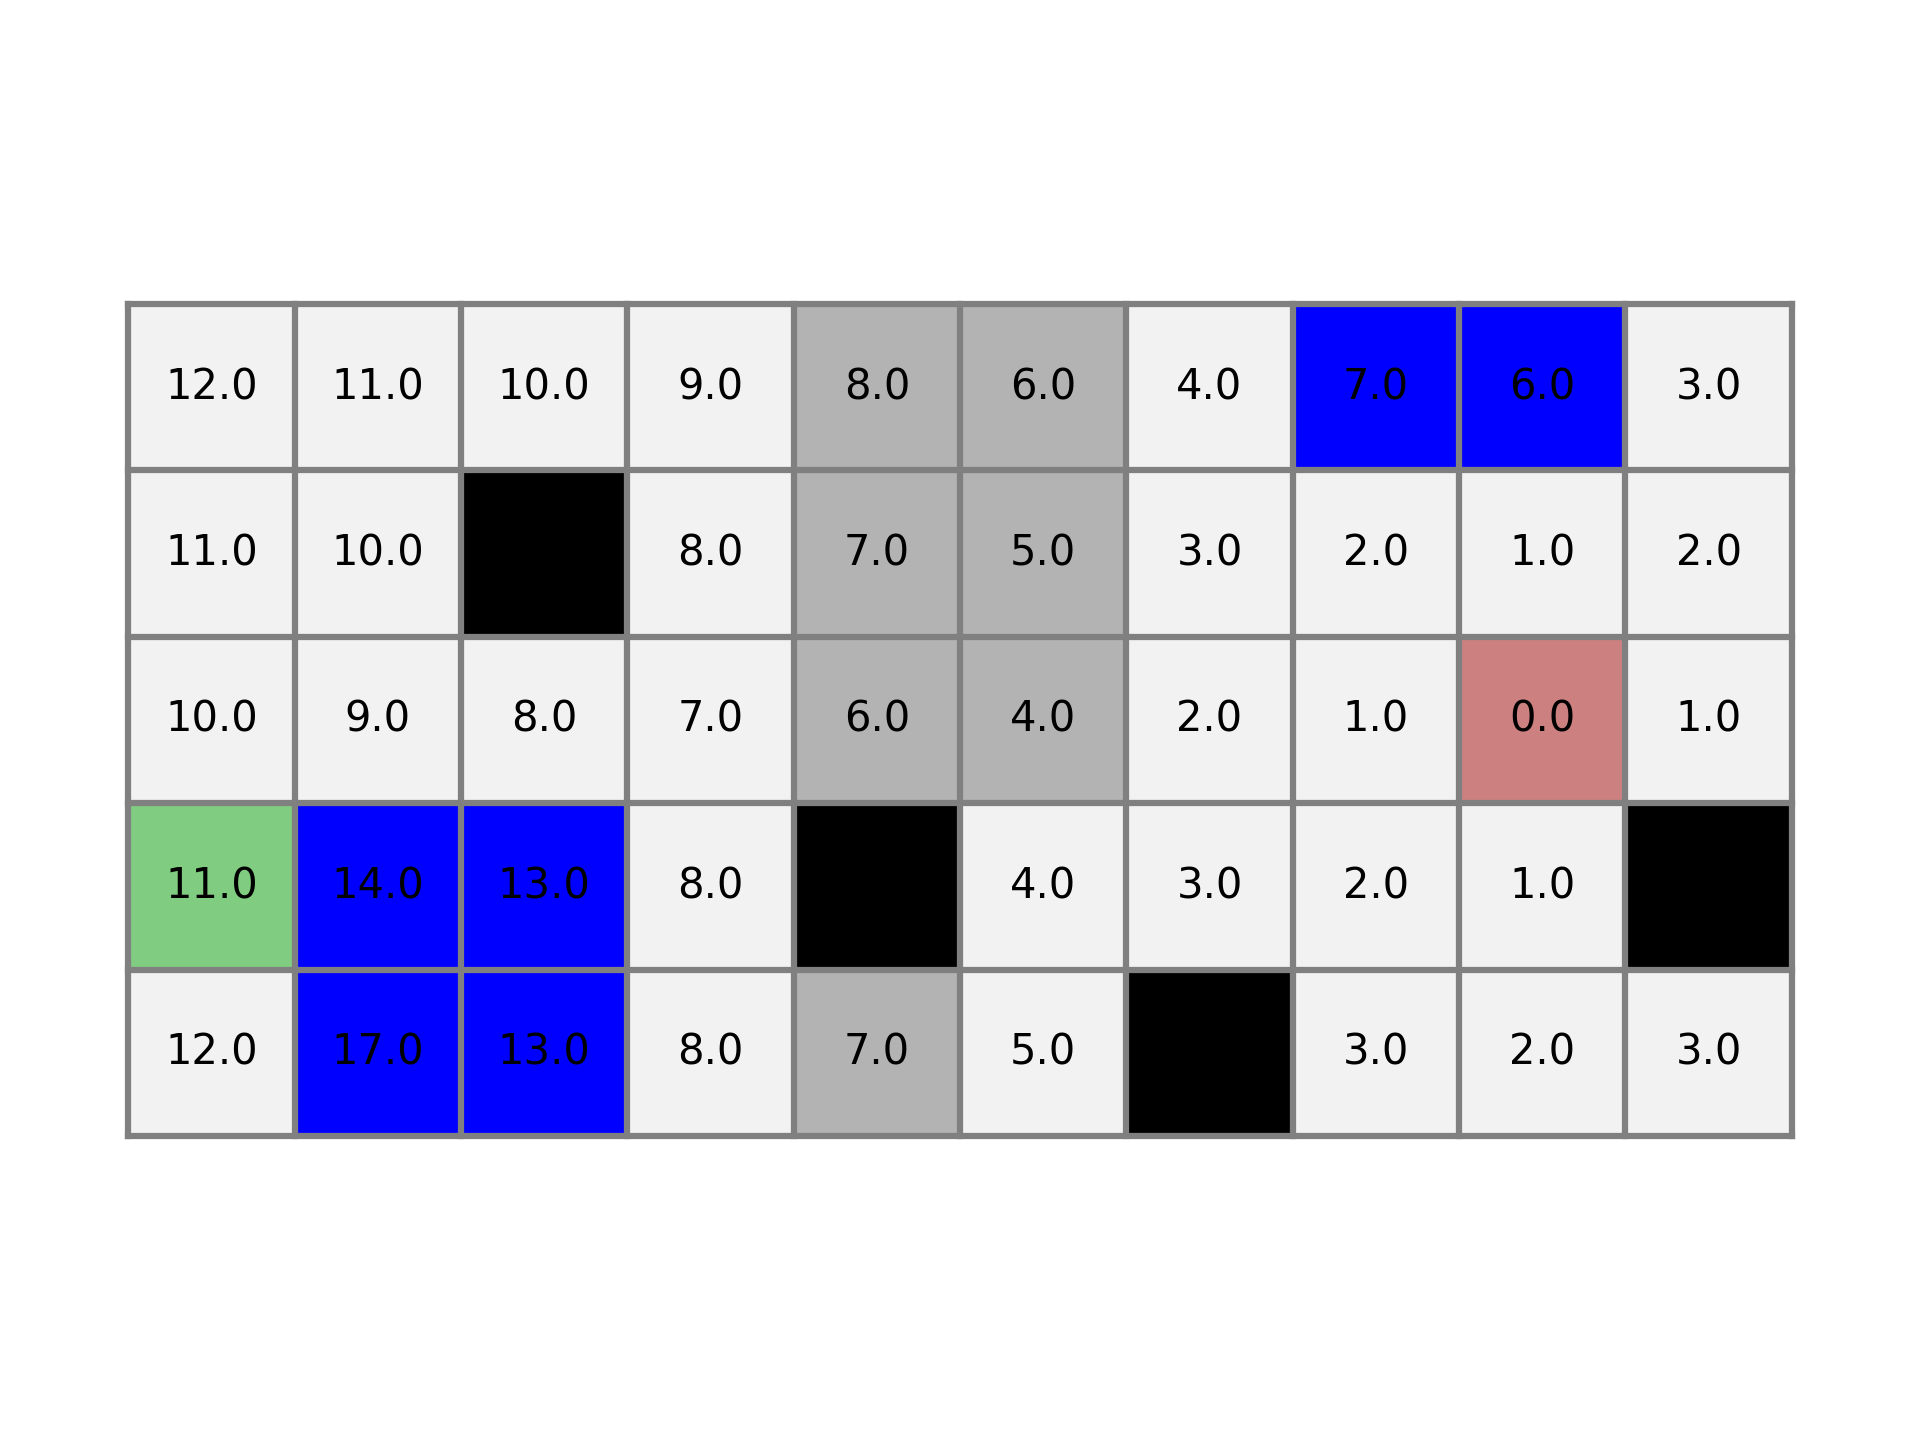
\includegraphics[scale=\myscale,scale=0.33,trim={0 2cm 0 2cm},clip]{figures/terrain-01-4}
	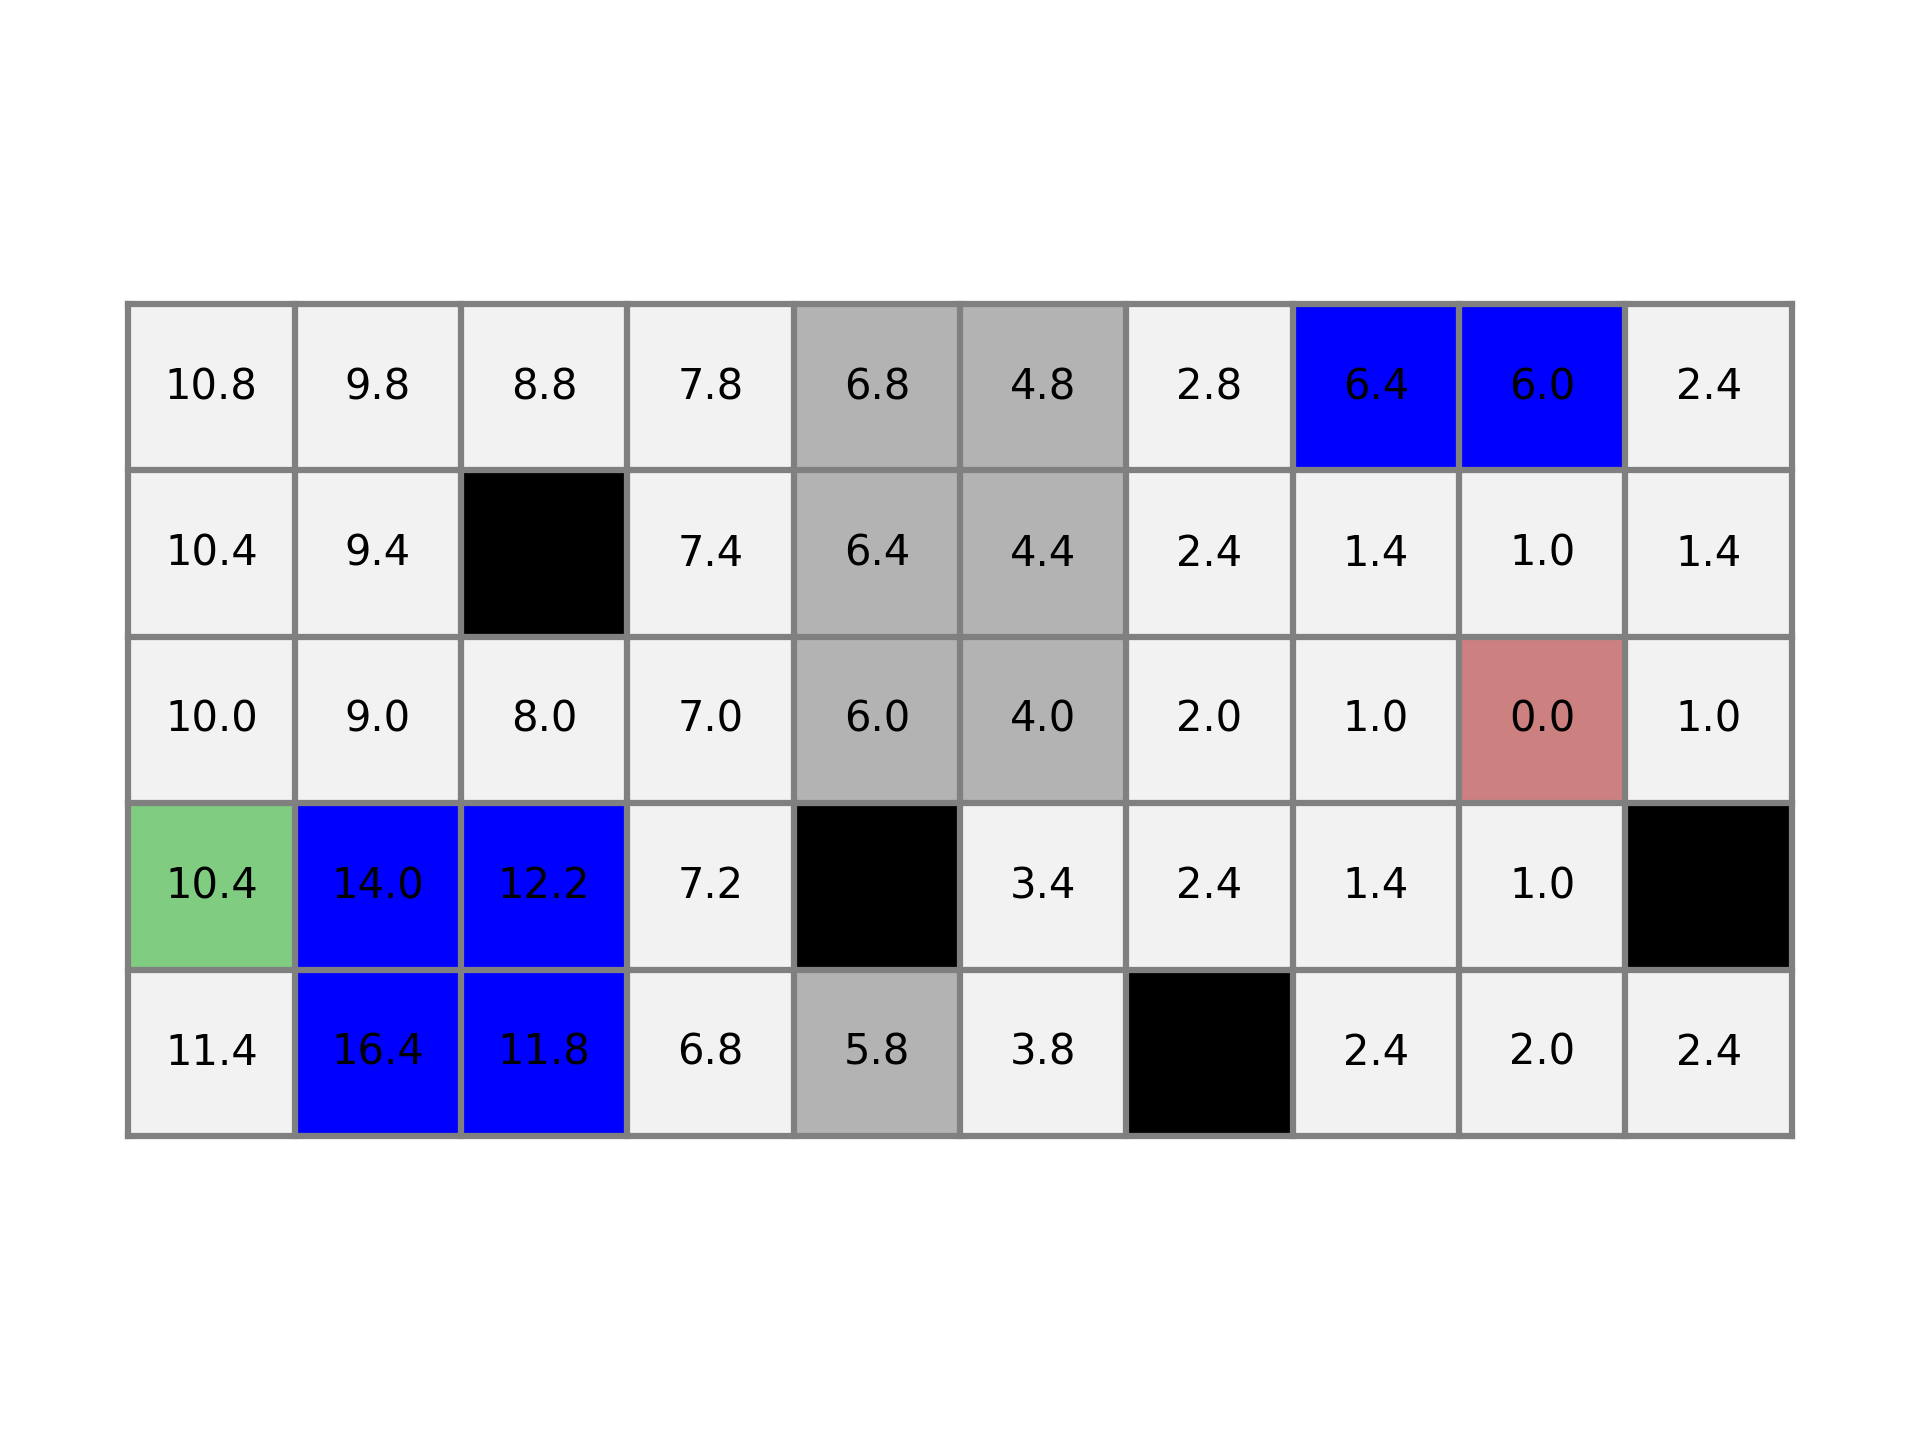
\includegraphics[scale=\myscale,scale=0.33,trim={0 2cm 0 2cm},clip]{figures/terrain-01-5}
	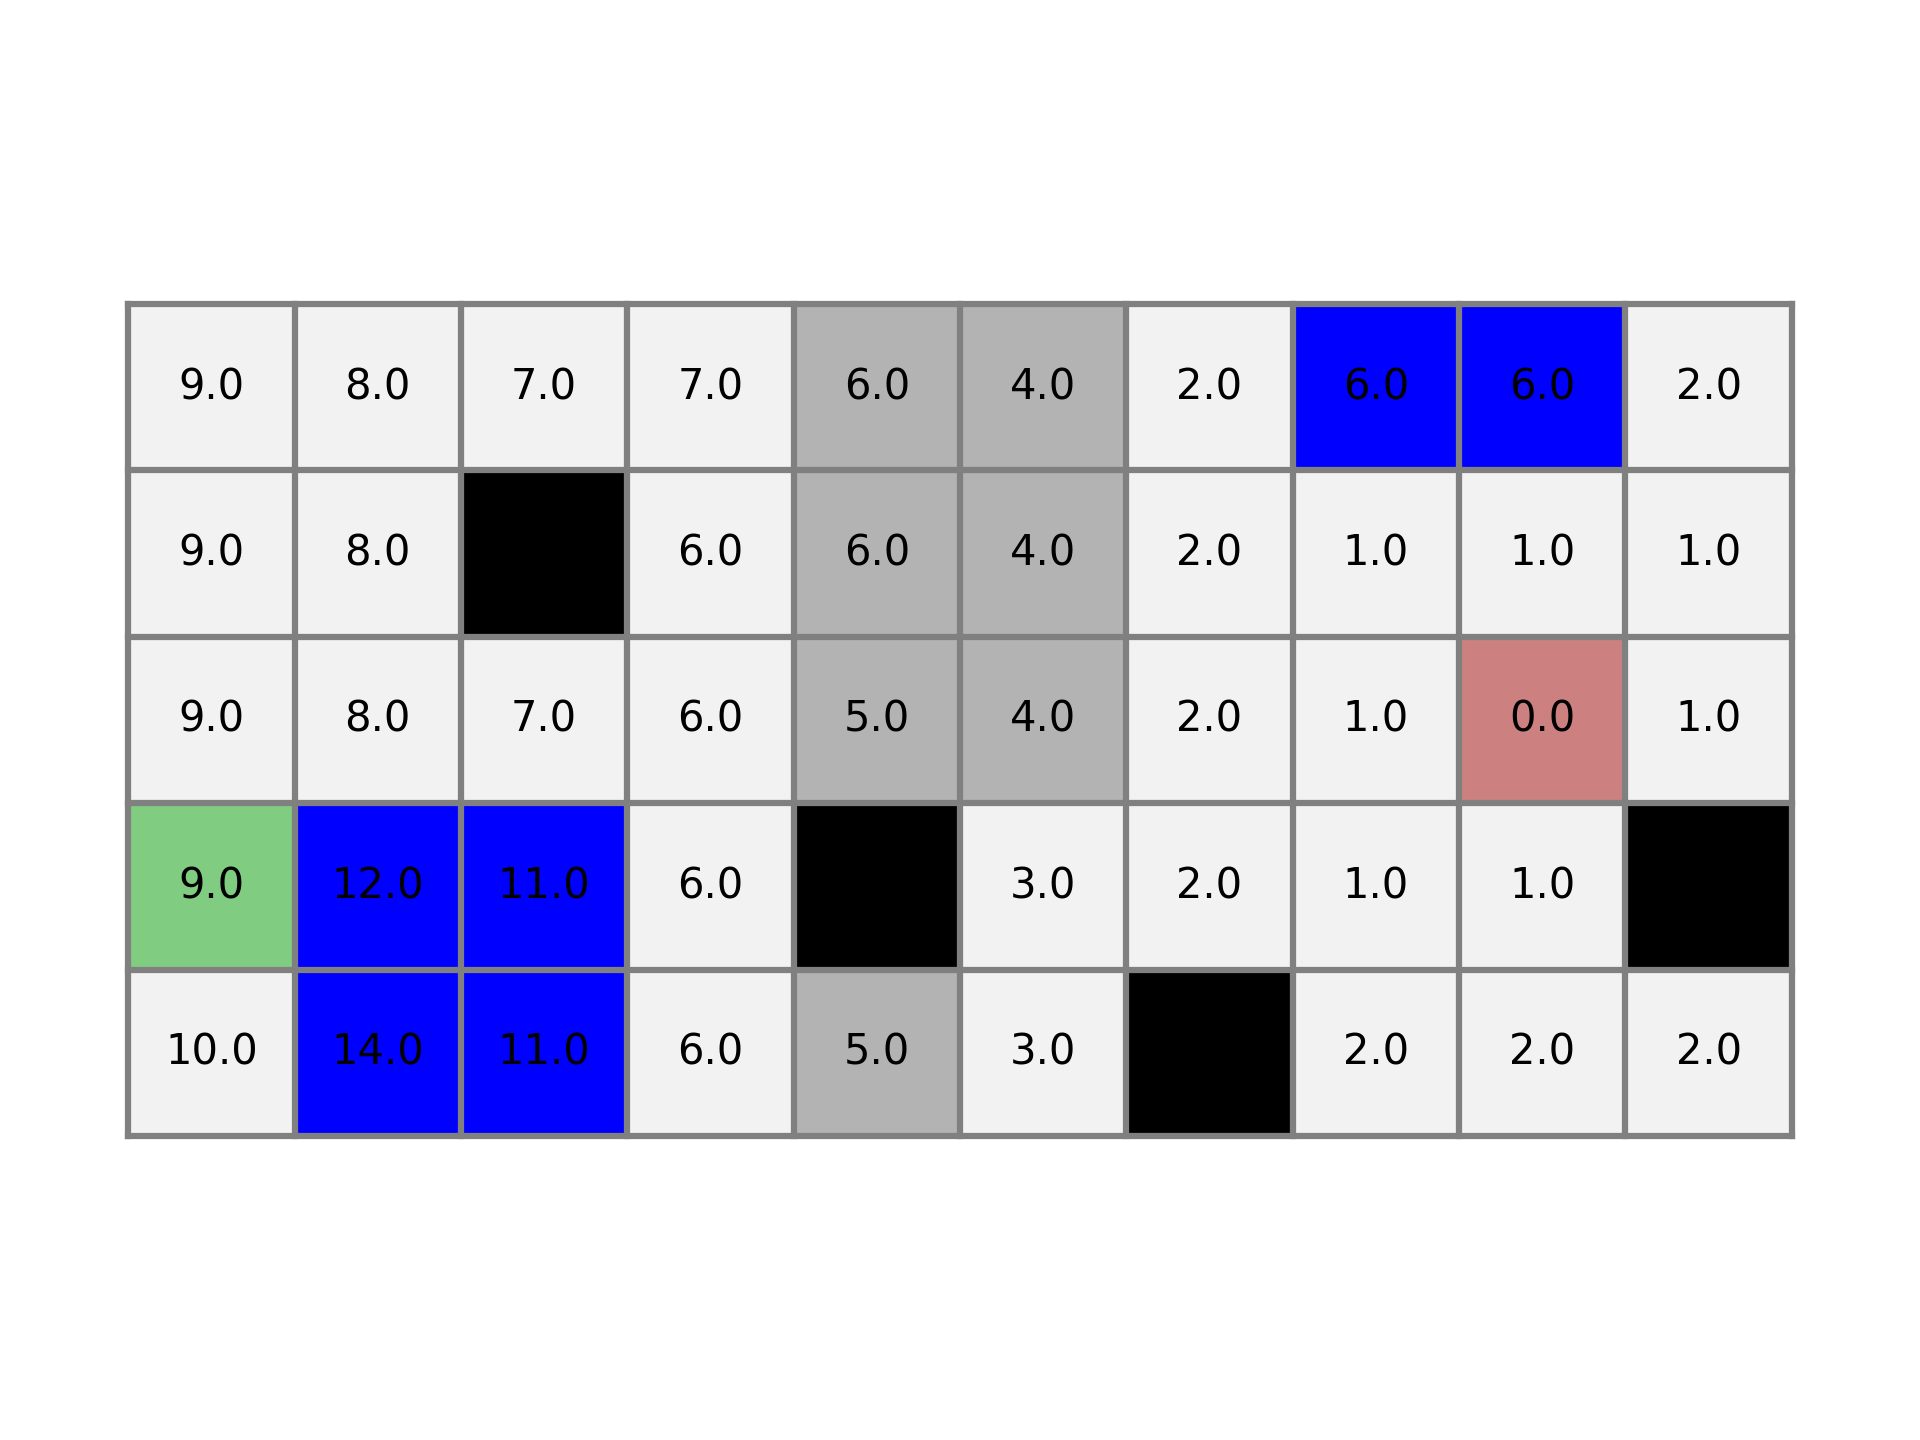
\includegraphics[scale=\myscale,scale=0.33,trim={0 2cm 0 2cm},clip]{figures/terrain-01-6}
\end{center}

Ci-dessous un exemple plus compliqué : à gauche le terrain, à droite la coloration de la \emph{heatmap} (pour la norme $1$).

\begin{center}
	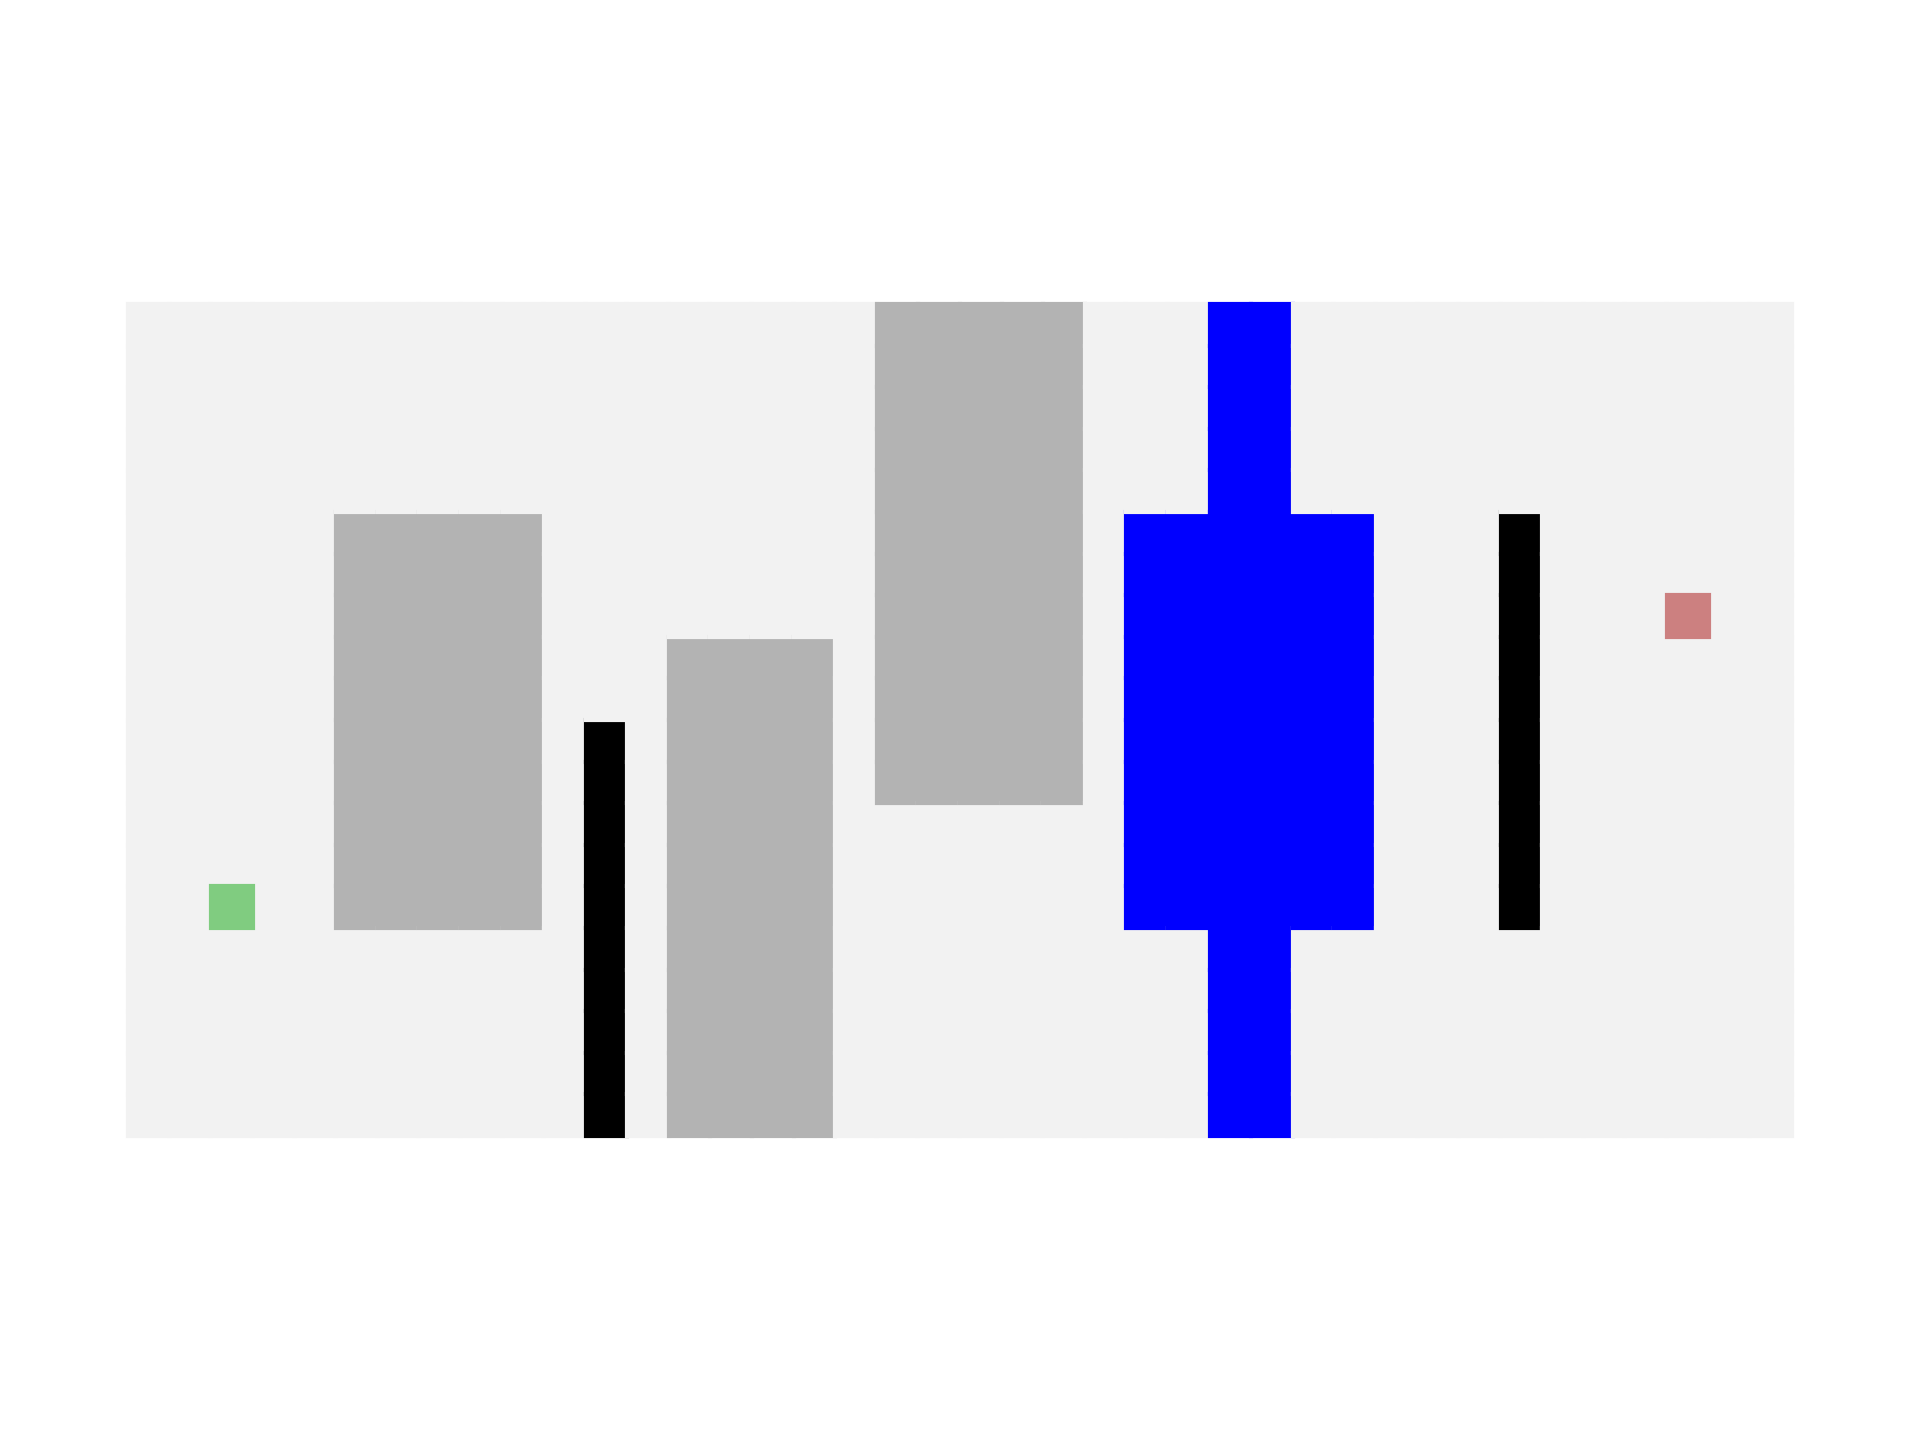
\includegraphics[scale=\myscale,scale=0.5,trim={0 2cm 0 2cm},clip]{figures/terrain-02-1}
	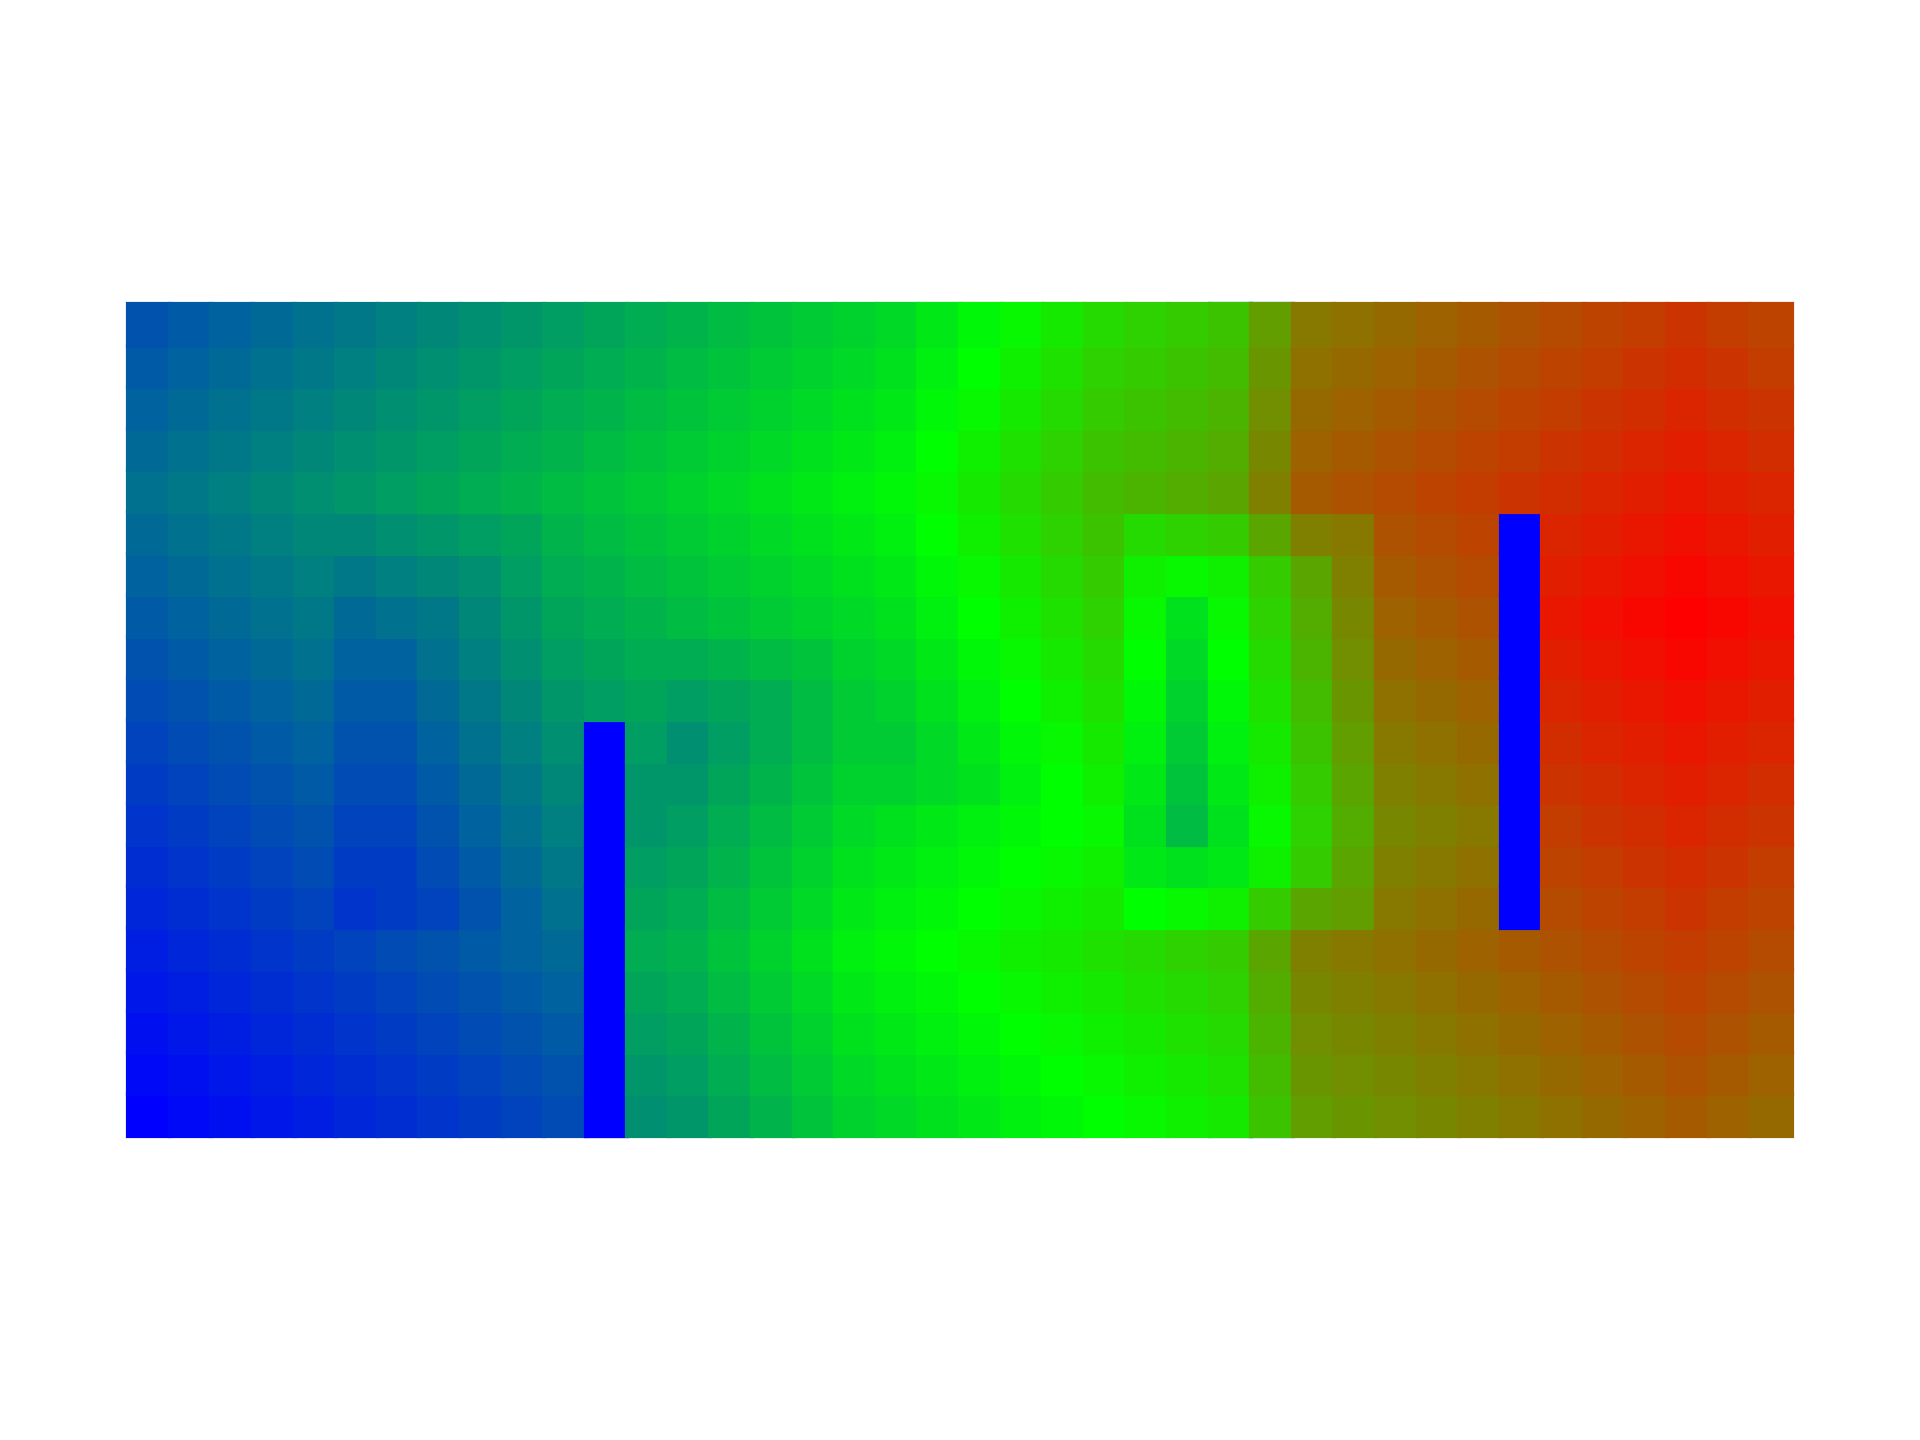
\includegraphics[scale=\myscale,scale=0.5,trim={0 2cm 0 2cm},clip]{figures/terrain-02-2}
\end{center}


%--------------------------------------------------------------------
\subsection{Chemin}

Comme dans le cas du labyrinthe, pour se diriger vers l'arrivée,
le plus simple est de chercher une case voisine avec la valeur de la \emph{heatmap} la plus petite possible.
Autrement dit à chaque case, une flèche indique la direction de la case voisine (y compris en diagonale) qui diminue le plus la distance vers l'arrivée. (S'il y a plusieurs cases qui réalisent ce minimum, on en prend une au hasard.)

\begin{center}
	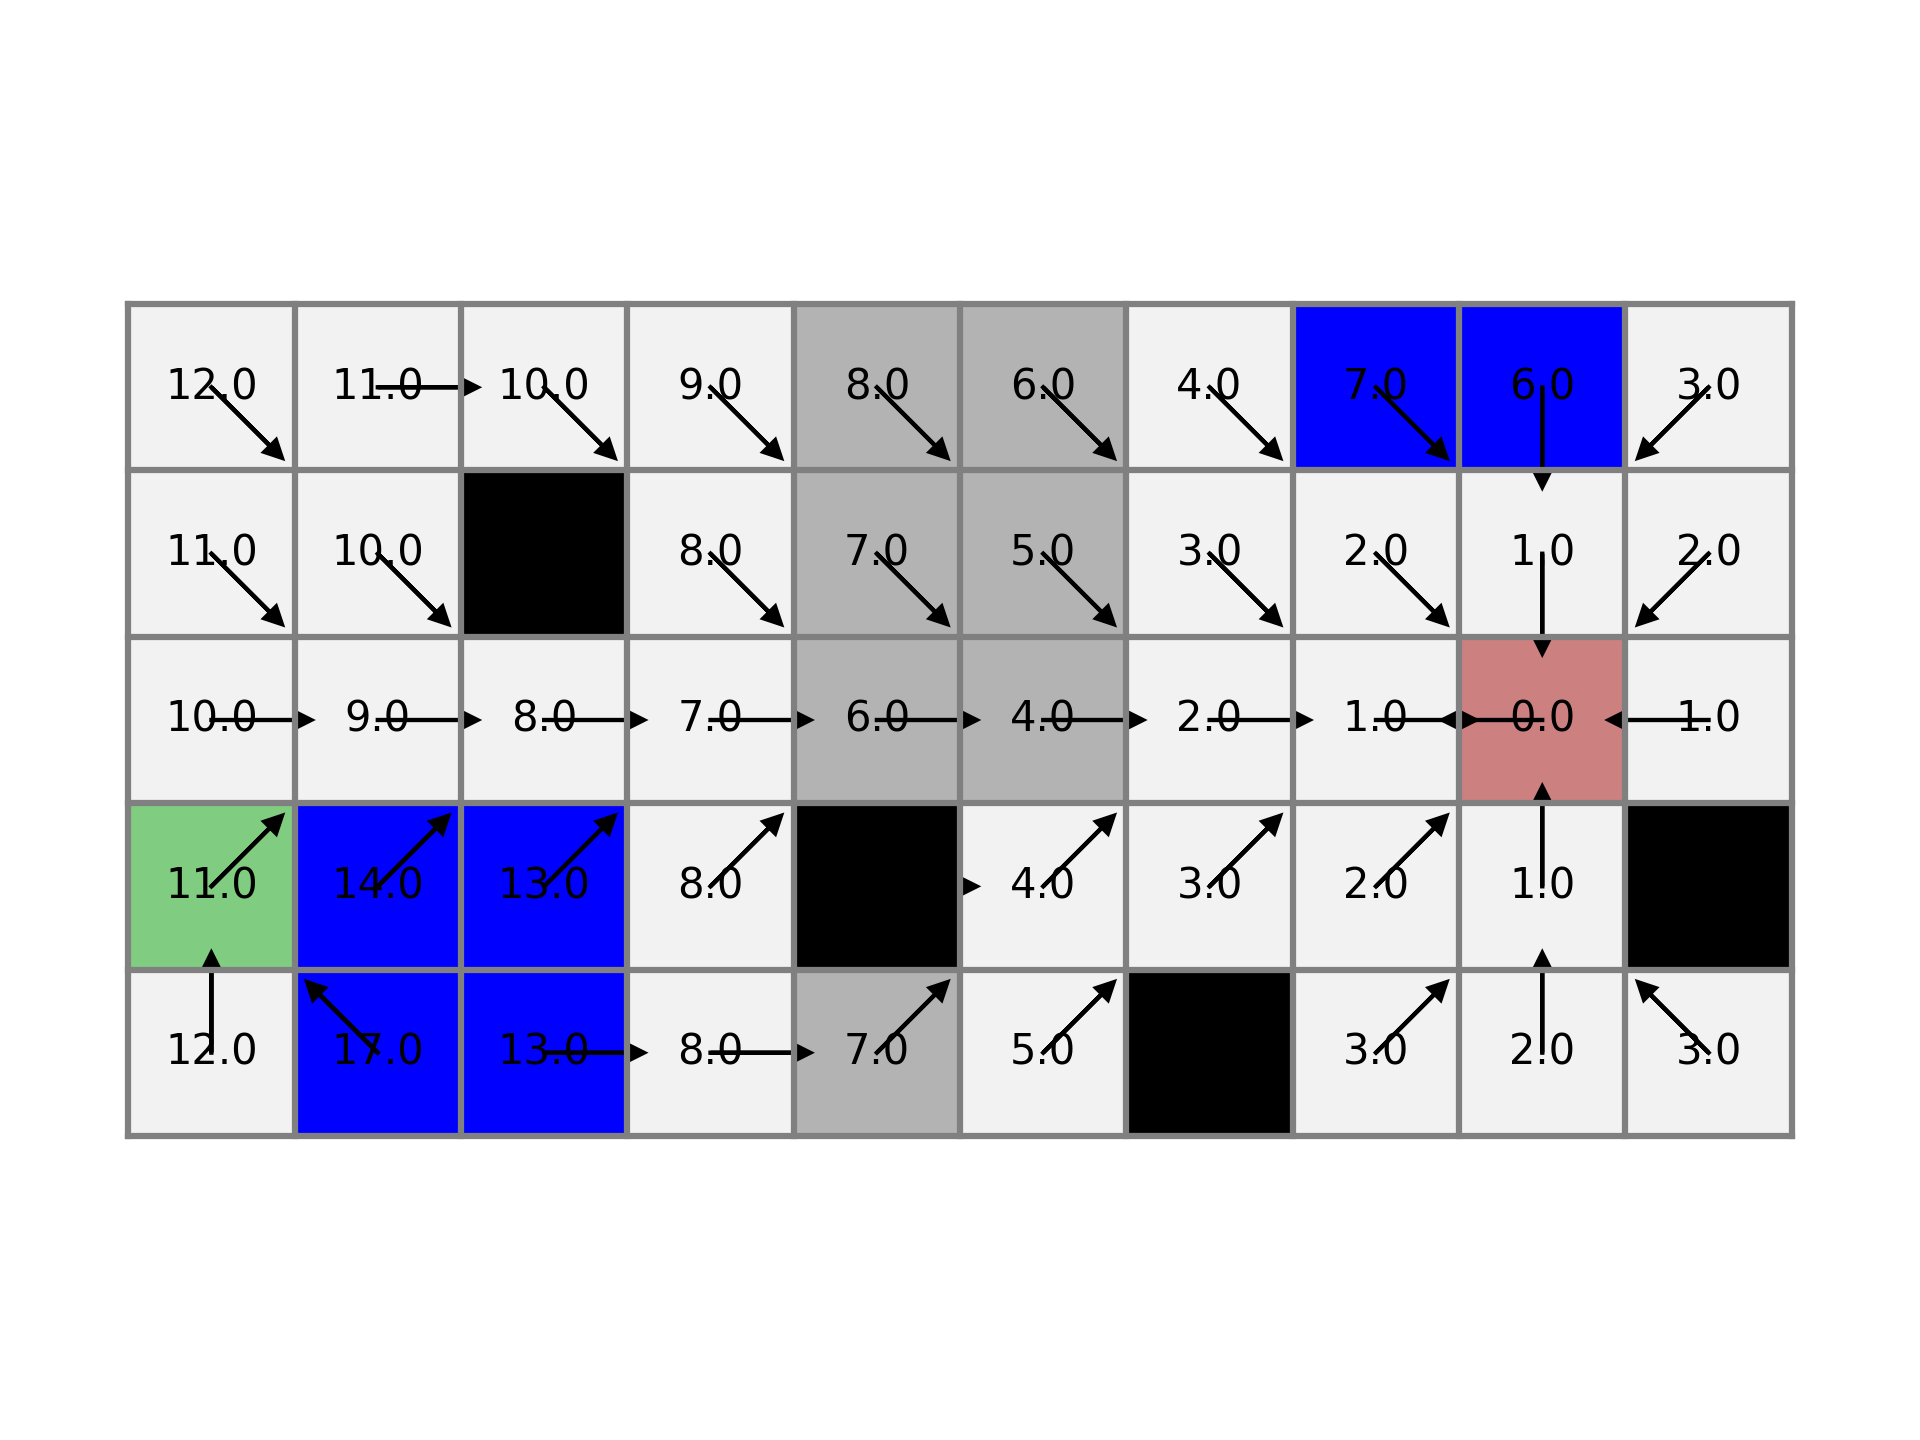
\includegraphics[scale=\myscale,scale=0.5,trim={0 2cm 0 2cm},clip]{figures/terrain-01-7}
\end{center}



%--------------------------------------------------------------------
\subsection{Gradient}

Avec la méthode du minimum, pour chaque case on obtient une direction parmi $8$ possibles (correspondant aux $8$ cases voisines), ce qui est assez limité. Comment obtenir plus de possibilités ?

Le \emph{gradient} d'une fonction $h$ de deux variables (ou plus) indique la direction de la plus forte pente, c'est-à-dire la direction à suivre pour passer à une valeur de $h$ la plus grande possible. C'est une version à deux dimensions de la dérivée.
Noter qu'ici on veut minimiser $h$, donc on va en fait suivre la direction opposée au gradient.

Nous allons calculer le gradient de $h$ en une case à l'aide d'une convolution vectorielle, c'est-à-dire qu'on va calculer un vecteur à l'aide de la grille $3\times3$ entourant la case.
Depuis la case centrale, de coordonnées $(0,0)$, on se déplace à une case $(i,j)$ voisine selon un vecteur $\vec{v_{ij}} = (i,j)$ où $i,j \in \{-1,0,1\}$. Par exemple $(1,0)$ désigne la case de droite et est associée au vecteur horizontal $(1,0)$.

En chaque case nous avons aussi une valeur $h(i,j)$ donnée par la \emph{heatmap}. Ce qui va intervenir c'est la différence entre la valeur $h_{00}$ en la case centrale et la valeur $h_{ij}$ en une case voisine.

Le gradient en $(0,0)$ se calcule selon la formule :
$$\vec{g} = \sum_{i,j}  (h_{ij} - h_{00}) \vec{v_{ij}} 
= (h_{10} - h_{00}) \begin{pmatrix}1\\0\end{pmatrix}
+ (h_{11} - h_{00}) \begin{pmatrix}1\\1\end{pmatrix}
+ (h_{01} - h_{00}) \begin{pmatrix}0\\1\end{pmatrix}
+ \cdots$$

\myfigure{0.7}{
	\tikzinput{fig-terrain-07}	
}

\begin{exemple}
Partons de cette mini-\emph{heatmap} (pour simplifier les calculs on a imposé $h_{00}=0$).	
\myfigure{0.7}{
	\tikzinput{fig-terrain-08}	
}
Le vecteur gradient associé à la case centrale est :
\begin{align*} 
\vec{g} &= 
(1)\times\rightarrow \ + \
(2)\times\nearrow \ + \ 
(1)\times\uparrow \ + \ 
(0)\times\nwarrow \ + \ 
(-1)\times\leftarrow \ + \ 
(-1)\times\swarrow \ + \ 
 (0)\times\downarrow  \ + \
(0)\times\searrow \\
 &= 
 1 \begin{pmatrix}1\\0\end{pmatrix}  
+2 \begin{pmatrix}1\\1\end{pmatrix} 
+1 \begin{pmatrix}0\\1\end{pmatrix}
-1 \begin{pmatrix}-1\\0\end{pmatrix}
-1 \begin{pmatrix}-1\\-1\end{pmatrix} 
 \\
 &=  \begin{pmatrix}5\\4\end{pmatrix}
\end{align*}
\end{exemple}

On se déplace ensuite vers la case indiquée par la direction $\vec g$.
Noter que si $h_{ij}> h_{00}$ on obtient une contribution dans le sens $\vec{v_{ij}}$ (on va donc se diriger vers des valeurs de $h$ plus hautes),  mais si $h_{ij} < h_{00}$ on obtient une contribution en sens inverse (on se dirige dans la direction opposées des valeurs plus basses).

Quelques ajustement peuvent être nécessaires, car ici notre fonction présente des sauts importants au niveau des obstacles et des terrains difficiles. On peut normaliser le vecteur $\vec g$ ou on peut modifier la formule par :
$$\vec{g} = \sum_{i,j}  \frac{1}{h_{ij} - h_{00}} \vec{v_{ij}}$$
(en omettant les termes où $h_{ij} = h_{00}$).

Les vecteurs obtenus par la méthode du gradient représentent mieux les spécificités du terrain que la méthode du minimum. On pourrait raffiner en calculant le gradient via une grille $5\times 5$ entourant chaque case. 
Ci-dessous à gauche, la direction indiquée par le minimum, à droite la direction opposée du gradient (normalisé).
\begin{center}
	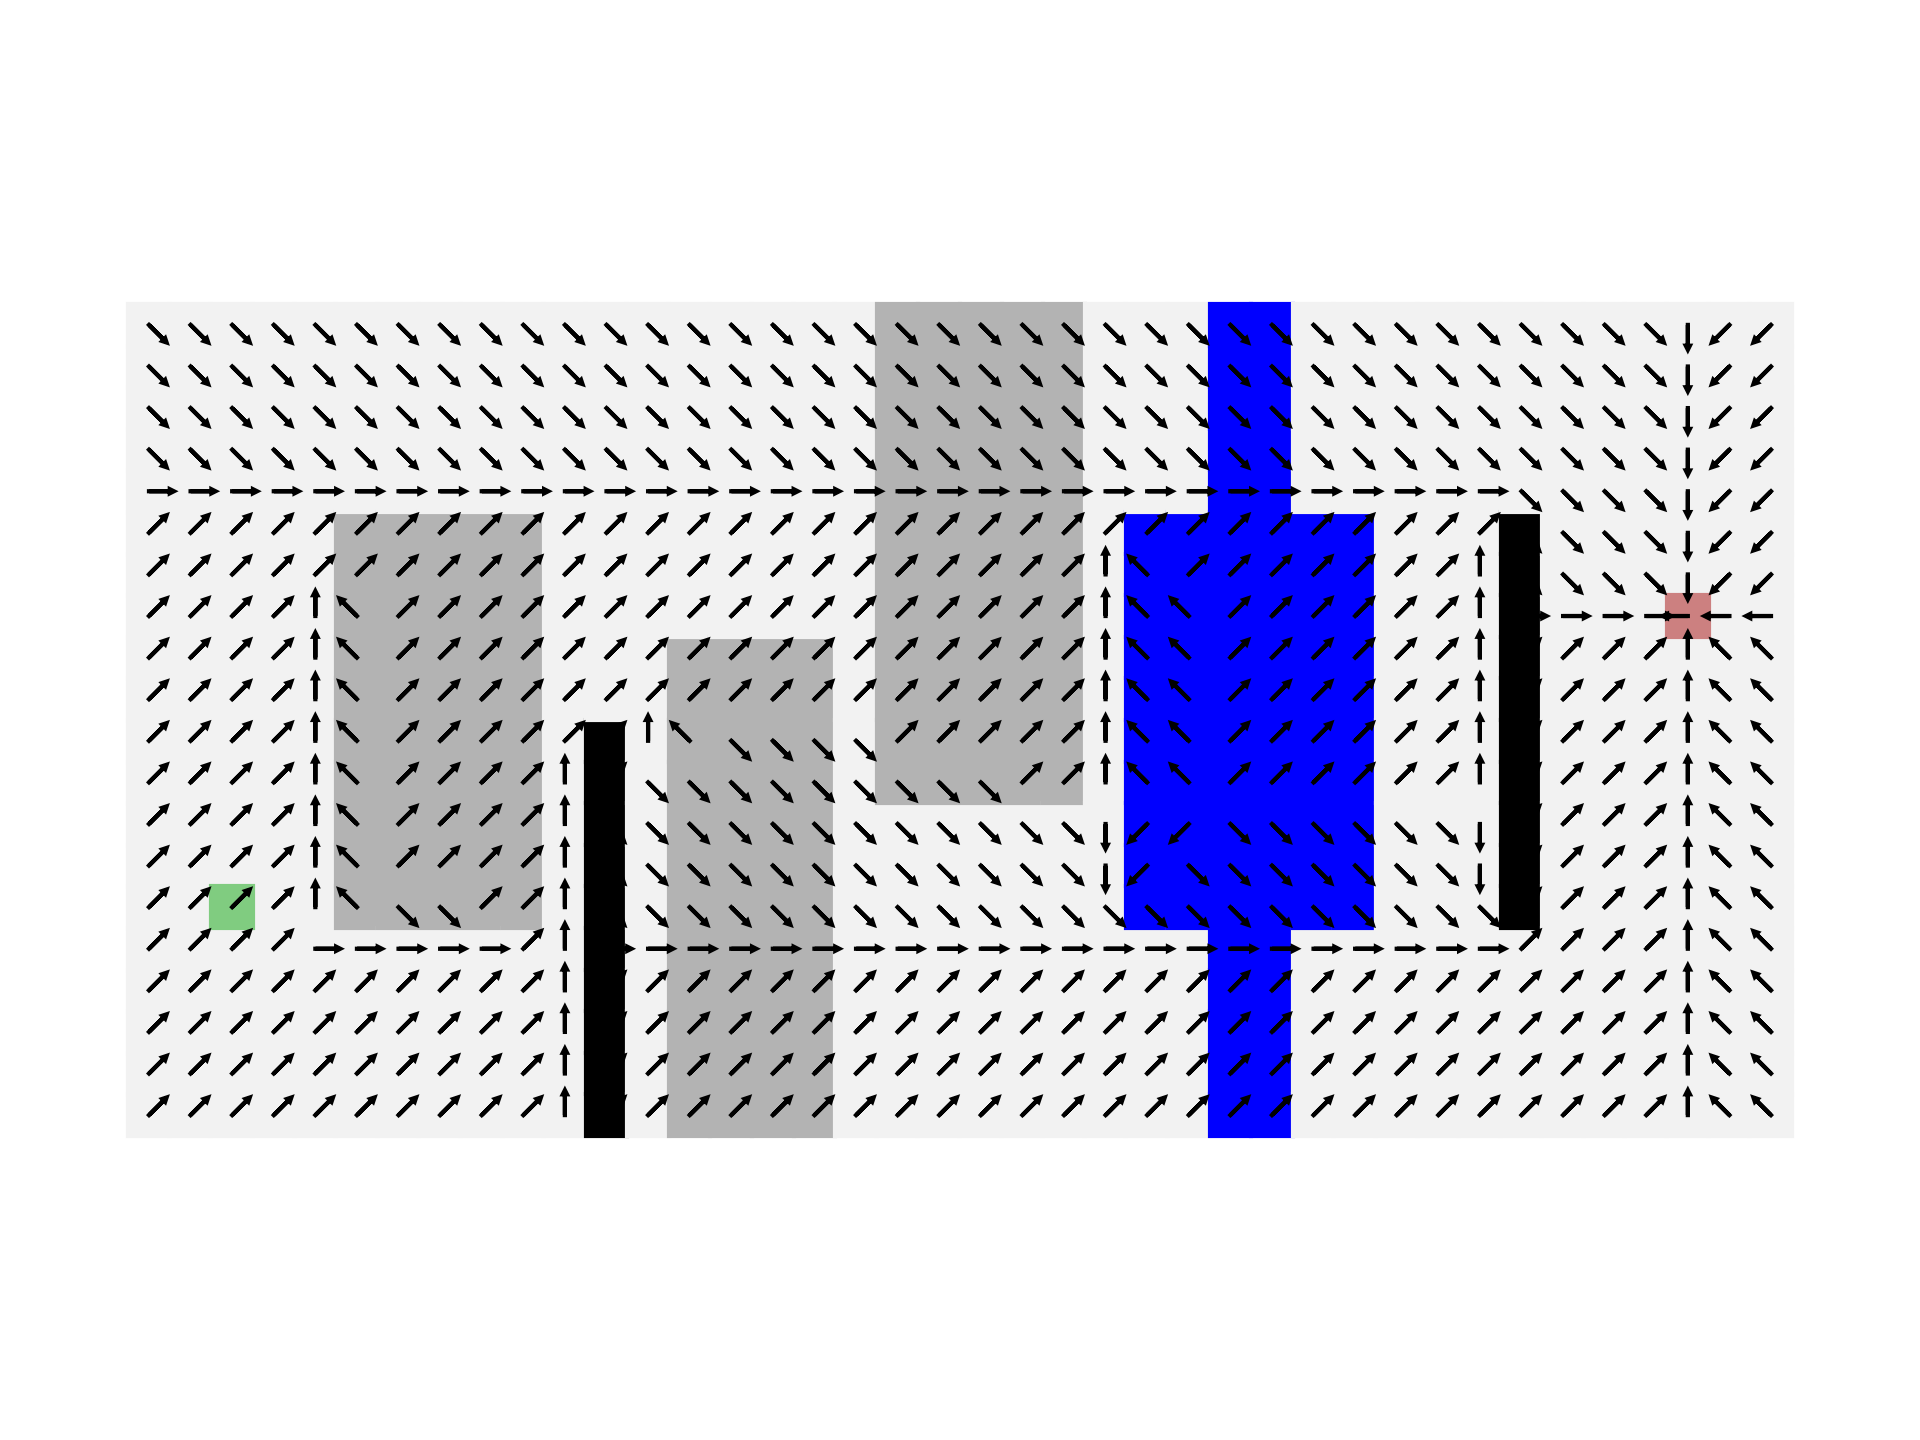
\includegraphics[scale=\myscale,scale=0.55,trim={1cm 2cm 0.5cm 2cm},clip]{figures/terrain-02-3}
	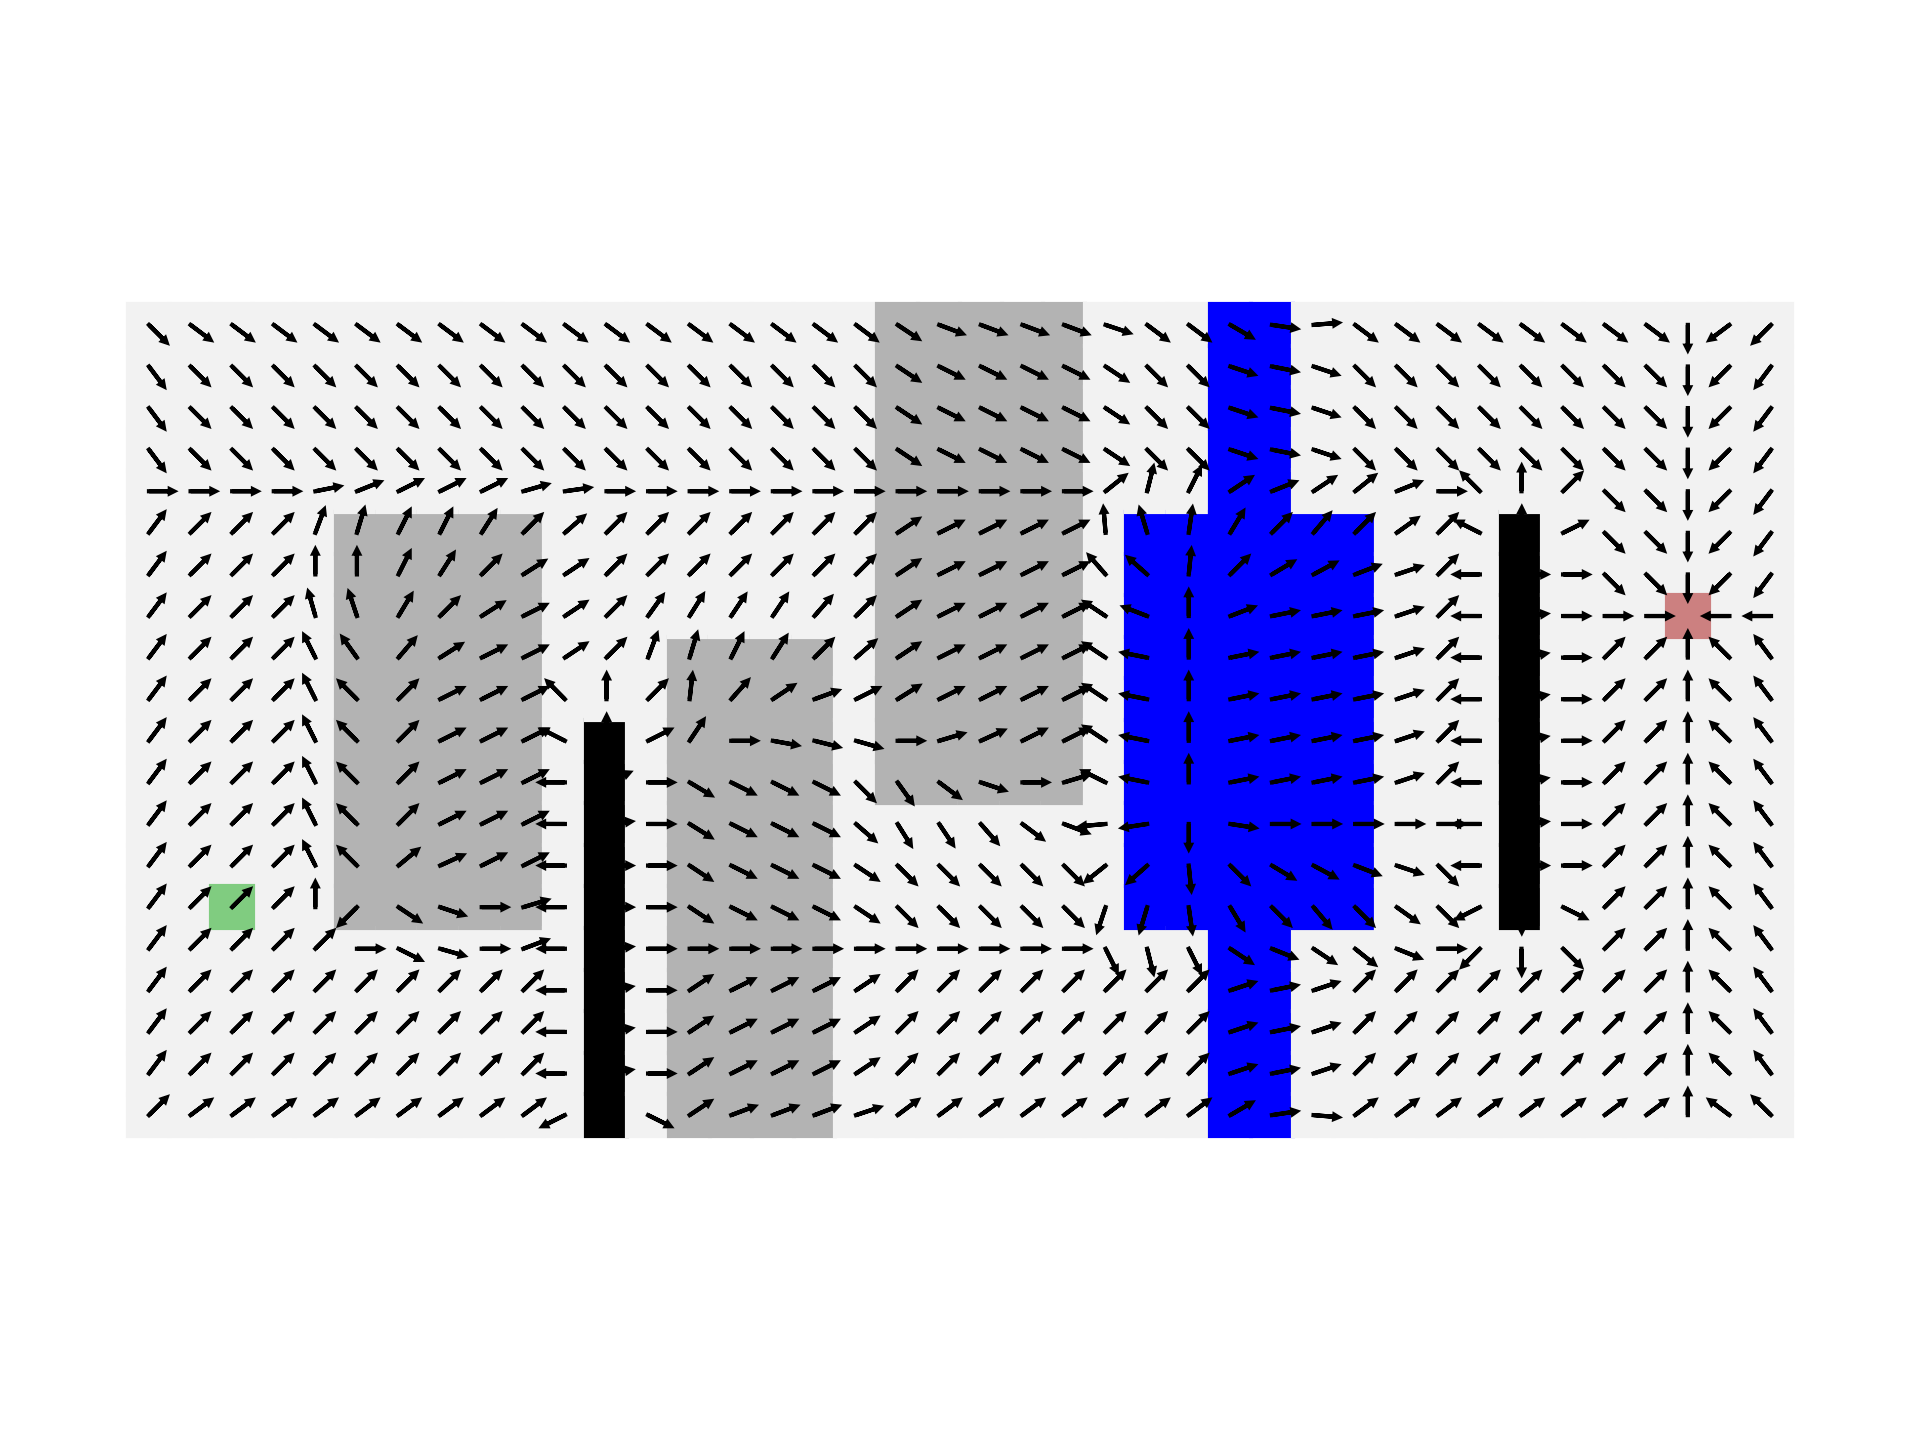
\includegraphics[scale=\myscale,scale=0.55,trim={0.5cm 2cm 1cm 2cm},clip]{figures/terrain-02-4}
\end{center}

\end{document}
